%%%%%%%%%%%%%%
%% Run LaTeX on this file several times to get Table of Contents,
%% cross-references, and citations.

%% If you have font problems, you may edit the w-bookps.sty file
%% to customize the font names to match those on your system.

%% w-bksamp.tex. Current Version: Feb 16, 2012
%%%%%%%%%%%%%%%%%%%%%%%%%%%%%%%%%%%%%%%%%%%%%%%%%%%%%%%%%%%%%%%%
%
%  Sample file for
%  Wiley Book Style, Design No.: SD 001B, 7x10
%  Wiley Book Style, Design No.: SD 004B, 6x9
%
%
%  Prepared by Amy Hendrickson, TeXnology Inc.
%  http://www.texnology.com
%%%%%%%%%%%%%%%%%%%%%%%%%%%%%%%%%%%%%%%%%%%%%%%%%%%%%%%%%%%%%%%%

%%%%%%%%%%%%%
% 7x10
%\documentclass{wileySev}

% 6x9
\documentclass{wileySix}

\usepackage{graphicx}
\usepackage{listings}
\usepackage{float}
\usepackage[urlcolor=blue, colorlinks=true]{hyperref}
\usepackage{textcomp}
\usepackage{color}
 
\definecolor{codegreen}{rgb}{0,0.6,0}
\definecolor{codegray}{rgb}{0.5,0.5,0.5}
\definecolor{codepurple}{rgb}{0.58,0,0.82}
\definecolor{backcolour}{rgb}{0.95,0.95,0.92}
 
\lstdefinestyle{mystyle}{
    backgroundcolor=\color{backcolour},   
    commentstyle=\color{codegreen},
    keywordstyle=\color{magenta},
    numberstyle=\tiny\color{codegray},
    stringstyle=\color{codepurple},
    basicstyle=\footnotesize,
    breakatwhitespace=false,         
    breaklines=true,                 
    captionpos=b,                    
    keepspaces=true,                 
    numbers=left,                    
    numbersep=5pt,                  
    showspaces=false,                
    showstringspaces=false,
    showtabs=false,                  
    tabsize=2,
    language=sh
}
 
\lstset{style=mystyle}

%%%%%%%
%% for times math: However, this package disables bold math (!)
%% \mathbf{x} will still work, but you will not have bold math
%% in section heads or chapter titles. If you don't use math
%% in those environments, mathptmx might be a good choice.

% \usepackage{mathptmx}

% For PostScript text
%\usepackage{w-bookps}

%%%%%%%%%%%%%%%%%%%%%%%%%%%%%%%%%%%%%%%%%%%%%%%%%%%%%%%%%%%%%%%%
%% Other packages you might want to use:

% for chapter bibliography made with BibTeX
% \usepackage{chapterbib}

% for multiple indices
% \usepackage{multind}

% for answers to problems
% \usepackage{answers}

%%%%%%%%%%%%%%%%%%%%%%%%%%%%%%
%% Change options here if you want:
%%
%% How many levels of section head would you like numbered?
%% 0= no section numbers, 1= section, 2= subsection, 3= subsubsection
%%==>>
\setcounter{secnumdepth}{3}

%% How many levels of section head would you like to appear in the
%% Table of Contents?
%% 0= chapter titles, 1= section titles, 2= subsection titles, 
%% 3= subsubsection titles.
%%==>>
\setcounter{tocdepth}{2}

%% Cropmarks? good for final page makeup
%% \docropmarks

%%%%%%%%%%%%%%%%%%%%%%%%%%%%%%
%
% DRAFT
%
% Uncomment to get double spacing between lines, current date and time
% printed at bottom of page.
% \draft
% (If you want to keep tables from becoming double spaced also uncomment
% this):
% \renewcommand{\arraystretch}{0.6}
%%%%%%%%%%%%%%%%%%%%%%%%%%%%%%

%%%%%%% Demo of section head containing sample macro:
%% To get a macro to expand correctly in a section head, with upper and
%% lower case math, put the definition and set the box 
%% before \begin{document}, so that when it appears in the 
%% table of contents it will also work:

\newcommand{\VT}[1]{\ensuremath{{V_{T#1}}}}

%% use a box to expand the macro before we put it into the section head:

\newbox\sectsavebox
\setbox\sectsavebox=\hbox{\boldmath\VT{xyz}}

%%%%%%%%%%%%%%%%% End Demo


\begin{document}


\booktitle{Cerdas Menguasai Git}
\subtitle{Dalam 24 Jam}

\authors{Rolly M. Awangga\\
\affil{Informatics Research Center}
%Floyd J. Fowler, Jr.\\
%\affil{University of New Mexico}
}

\offprintinfo{Cerdas Menguasai Git, First Edition}{Rolly M. Awangga}

%% Can use \\ if title, and edition are too wide, ie,
%% \offprintinfo{Survey Methodology,\\ Second Edition}{Robert M. Groves}

%%%%%%%%%%%%%%%%%%%%%%%%%%%%%%
%% 
\halftitlepage

\titlepage


\begin{copyrightpage}{2019}
%Survey Methodology / Robert M. Groves . . . [et al.].
%\       p. cm.---(Wiley series in survey methodology)
%\    ``Wiley-Interscience."
%\    Includes bibliographical references and index.
%\    ISBN 0-471-48348-6 (pbk.)
%\    1. Surveys---Methodology.  2. Social 
%\  sciences---Research---Statistical methods.  I. Groves, Robert M.  II. %
%Series.\\
%
%HA31.2.S873 2007
%001.4'33---dc22                                             2004044064
\end{copyrightpage}

\dedication{`Jika Kamu tidak dapat menahan lelahnya belajar, 
Maka kamu harus sanggup menahan perihnya Kebodohan.'
~Imam Syafi'i~}

\begin{contributors}
\name{Rolly Maulana Awangga,} Informatics Research Center., Politeknik Pos Indonesia, Bandung,
Indonesia



\end{contributors}

\contentsinbrief
\tableofcontents
\listoffigures
\listoftables
\lstlistoflistings


\begin{foreword}
Sepatah kata dari Kaprodi, Kabag Kemahasiswaan dan Mahasiswa
\end{foreword}

\begin{preface}
Buku ini diciptakan bagi yang awam dengan git sekalipun.

\prefaceauthor{R. M. Awangga}
\where{Bandung, Jawa Barat\\
Februari, 2019}
\end{preface}


\begin{acknowledgments}
Terima kasih atas semua masukan dari para mahasiswa agar bisa membuat buku ini 
lebih baik dan lebih mudah dimengerti.

Terima kasih ini juga ditujukan khusus untuk team IRC yang 
telah fokus untuk belajar dan memahami bagaimana buku ini mendampingi proses 
Intership.
\authorinitials{R. M. A.}
\end{acknowledgments}

\begin{acronyms}
\acro{ACGIH}{American Conference of Governmental Industrial Hygienists}
\acro{AEC}{Atomic Energy Commission}
\acro{OSHA}{Occupational Health and Safety Commission}
\acro{SAMA}{Scientific Apparatus Makers Association}
\end{acronyms}

\begin{glossary}
\term{git}Merupakan manajemen sumber kode yang dibuat oleh linus torvald.

\term{bash}Merupakan bahasa sistem operasi berbasiskan *NIX.

\term{linux}Sistem operasi berbasis sumber kode terbuka yang dibuat oleh Linus Torvald
\end{glossary}

\begin{symbols}
\term{A}Amplitude

\term{\hbox{\&}}Propositional logic symbol 

\term{a}Filter Coefficient

\bigskip

\term{\mathcal{B}}Number of Beats
\end{symbols}

\begin{introduction}

%% optional, but if you want to list author:

\introauthor{Rolly Maulana Awangga, S.T., M.T.}
{Informatics Research Center\\
Bandung, Jawa Barat, Indonesia}

Pada era disruptif  \index{disruptif}\index{disruptif!modern} 
saat ini. git merupakan sebuah kebutuhan dalam sebuah organisasi pengembangan perangkat lunak.
Buku ini diharapkan bisa menjadi penghantar para programmer, analis, IT Operation dan Project Manajer.
Dalam melakukan implementasi git pada diri dan organisasinya.

Rumusnya cuman sebagai contoh aja biar keren\cite{awangga2018sampeu}.

\begin{equation}
ABC {\cal DEF} \alpha\beta\Gamma\Delta\sum^{abc}_{def}
\end{equation}

\end{introduction}

%%%%%%%%%%%%%%%%%%Isi Buku_

\chapter{Chapter 1}
\section{1174006 - Kadek Diva Krishna Murti}
Lorem ipsum dolor sit amet, consectetur adipiscing elit.

\lstinputlisting[firstline=1, lastline=8]{references.bib}
\hfill\break
\begin{figure}[H]
    
\includegraphics[width=4cm]{kreatiflogo.png}
    \centering
    \caption{Kecerdasan Buatan.}
\end{figure}

\begin{enumerate}
	\item Lorem ipsum dolor sit amet, consectetur adipiscing elit.
	\item Lorem ipsum dolor sit amet, consectetur adipiscing elit.
	\item Lorem ipsum dolor sit amet, consectetur adipiscing elit.
\end{enumerate}

\subsection{Teori}

\subsection{Praktek}

\subsection{Penanganan Error}

\subsection{Bukti Tidak Plagiat}
\begin{figure}[H]
	
\includegraphics[width=4cm]{kreatiflogo.png}
	\centering
	\caption{Kecerdasan Buatan.}
\end{figure}
\section{1174035 - Luthfi Muhammad Nabil}
Kecerdasan buatan merupakan kecerdasan yang dimasukkan ke sistem yang dapat diatur untuk kepentingan ilmiah. Kecerdasan buatan biasa disebut AI (Artificial Intelligence) yang didefinisikan sebagai kecerdasan ilmiah. AI memiliki kemampuan untuk menerjemahkan data dari luar, dan mempelajari data tersebut untuk dipelajari demi mencapai tujuan dan melakukan tugas tertentu sesuai hasil adaptasi berdasarkan data yang didapat. 

\subsection{Sejarah dan perkembangan Kecerdasan Buatan}
AI mulai berkembang sesuai dengan konsep yang dikemukakan pada awal abad 17, Rene Descartes menyebutkan bahwa tubuh hewan bukanlah apa-apa melainkan mesin-mesin yang rumit. Lalu Blaise Pascal menciptakan mesin perhitungan digital mekanis pertama pada 1642. Selanjutnya pada abad ke 19, Charles Babbage dan Ada Lovelace menciptakan sebuah mesin penghitung mekanis yang dapat diprogram.

Pada tahun 1950-an, Program AI pertama yang sudah dapat difungsikan telah ditulis pada 1951 untuk menjalankan mesin Ferranti Mark I di University of Manchester yang merupakan sebuah program permainan naskah yang ditulis oleh Christopher Strachey. John McCarthy menyebutkan istilah "kecerdasan buatan" pada konferensi pertama yang disediakan untuk persoalan ini. Dilanjut pada tahun 1956, Beliau menemukan bahasa pemrograman yang bernama Lisp.

Jaringan saraf mulai digunakan secara luas pada tahun 1980-an, dimana algoritma perambatan balik pertama kali dijelaskan oleh Paul John Werbos pada tahun 1974. Selanjutnya di tahun 1982, para ahli fisika menganalisis sifat dari penyimpanan dan optimasi pada jaringan saraf menggunakan sistem statistika. Lalu dilanjutkan pada tahun 1985 sedikitnya empat kelompok riset menemukan algoritma pembelajaran propagansi balik. Algoritma ini berhasil diimplementasikan ke ilmu komputer dan psikologi. Dan pada tahun 1990, ditandai perolehan besar dalam berbagai bidang AI dan demonstrasi dari berbagai aplikasi yang sudah mengimplementasi. Seperti Deep Blue, sebuah komputer dari permainan catur yang dapat mengalahkan Garry Kasparov dalam sebuah pertandingan 6 game yang terkenal pada 1997. 

\subsection{Supervised Learning}
Supervised learning adalah kondisi yang menggunakan variabel input dan output untuk dapat dilakukan pemetaan input output yang sudah didapat. Disebud Supervised Learning karena proses dari pembelajaran algoritma dari pembelajan yang disumberkan dengan dataset dapat dipikirkan seperti seorang guru yang mengawasi proses pembelajaran. Proses pembelajaran dari algoritma akan berhenti saat algoritma sudah mendapatkan level dari performansi yang dapat diterima.
\hfill\break
Masalah dari Supervised learning dapat dikelompokkan menjadi masalah dengan regresi dan klasifikasi
\begin{itemize}
	\item Klasifikasi : Masalah dalam klasifikasi yang dimana output dari variable itu adalah kategori, seperti "Laki - laki" atau "Perempuan, dan "Muda" dan "Tua"
	\item Regresi : Masalah dalam regresi adalah jika pengeluaran dari variabel adalah sebuah nilai asli, seperti "suhu", dan "tinggi"
\end{itemize}

\subsection{Unsupervised Learning}
Unsupervised learning adalah kondisi dimana kamu hanya memiliki input data tanpa memiliki variabel output yang sesuai. Tujuan dari unsupervised learning adalah untuk memodelkan distribusi pada data untuk mengetahui lebih lanjut mengenai data. Disebut unsupervised learning karena pada metode ini, tidak ada jawaban yang tepat dan tidak ada pengarah. Sehingga algoritma akan ditinggalkan sesuai rancangan demi menemukan dan dapat mengolah data yang menarik pada saat yang akan datang. 

\subsection{Jenis - Jenis Dataset}
Dataset merupakan objek yang merepresentasikan data dan relasinya di memor. Strukturnya dapat mirip sesuai dengan struktur yang ada pada database namun bisa diubah sesuai dengan kebutuhan. Dataset juga berisi koleksi dari tabel data dan relasi data.
\begin{itemize}
	\item Training set : merupakan sebuah dataset yang digunakan untuk kepentingan pembelajaran. Kepentingan tersebut akan disesuaikan dengan parameter yang ada. 
	\item Test dataset : adalah sebuah dataset yang bersifat independen dibandingkan dengan training dataset, namun mengikuti probabilitas distribusi yang sama dengan training dataset. Jika model sudah sesuai dengan training dataset maka dataset sudah dapat disesuaikan dengan test dataset. Penyesuaian dari training dataset .
\end{itemize}

\subsection{Instalasi dan Percobaan Kompilasi dari Library Scikit-learn}
\begin{enumerate}
	\item Buka anaconda prompt
	\item Ketik di anaconda prompt yaitu : "pip install -U scikit-learn" untuk instalasi \hfill \break
	\begin{figure}[H]
		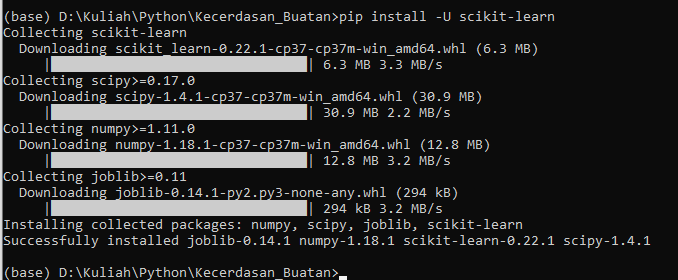
\includegraphics[width=4cm]{figures/1174035/chapter1/1_1.png}
		\centering
		\caption{Instalasi Scikit Learn}
	\end{figure}
	\item Setelah selesai instalasi, pilih salah satu example dari website Scikit (Contoh : \href{https://scikit-learn.org/stable/auto_examples/index.html})
	\begin{figure}[H]
		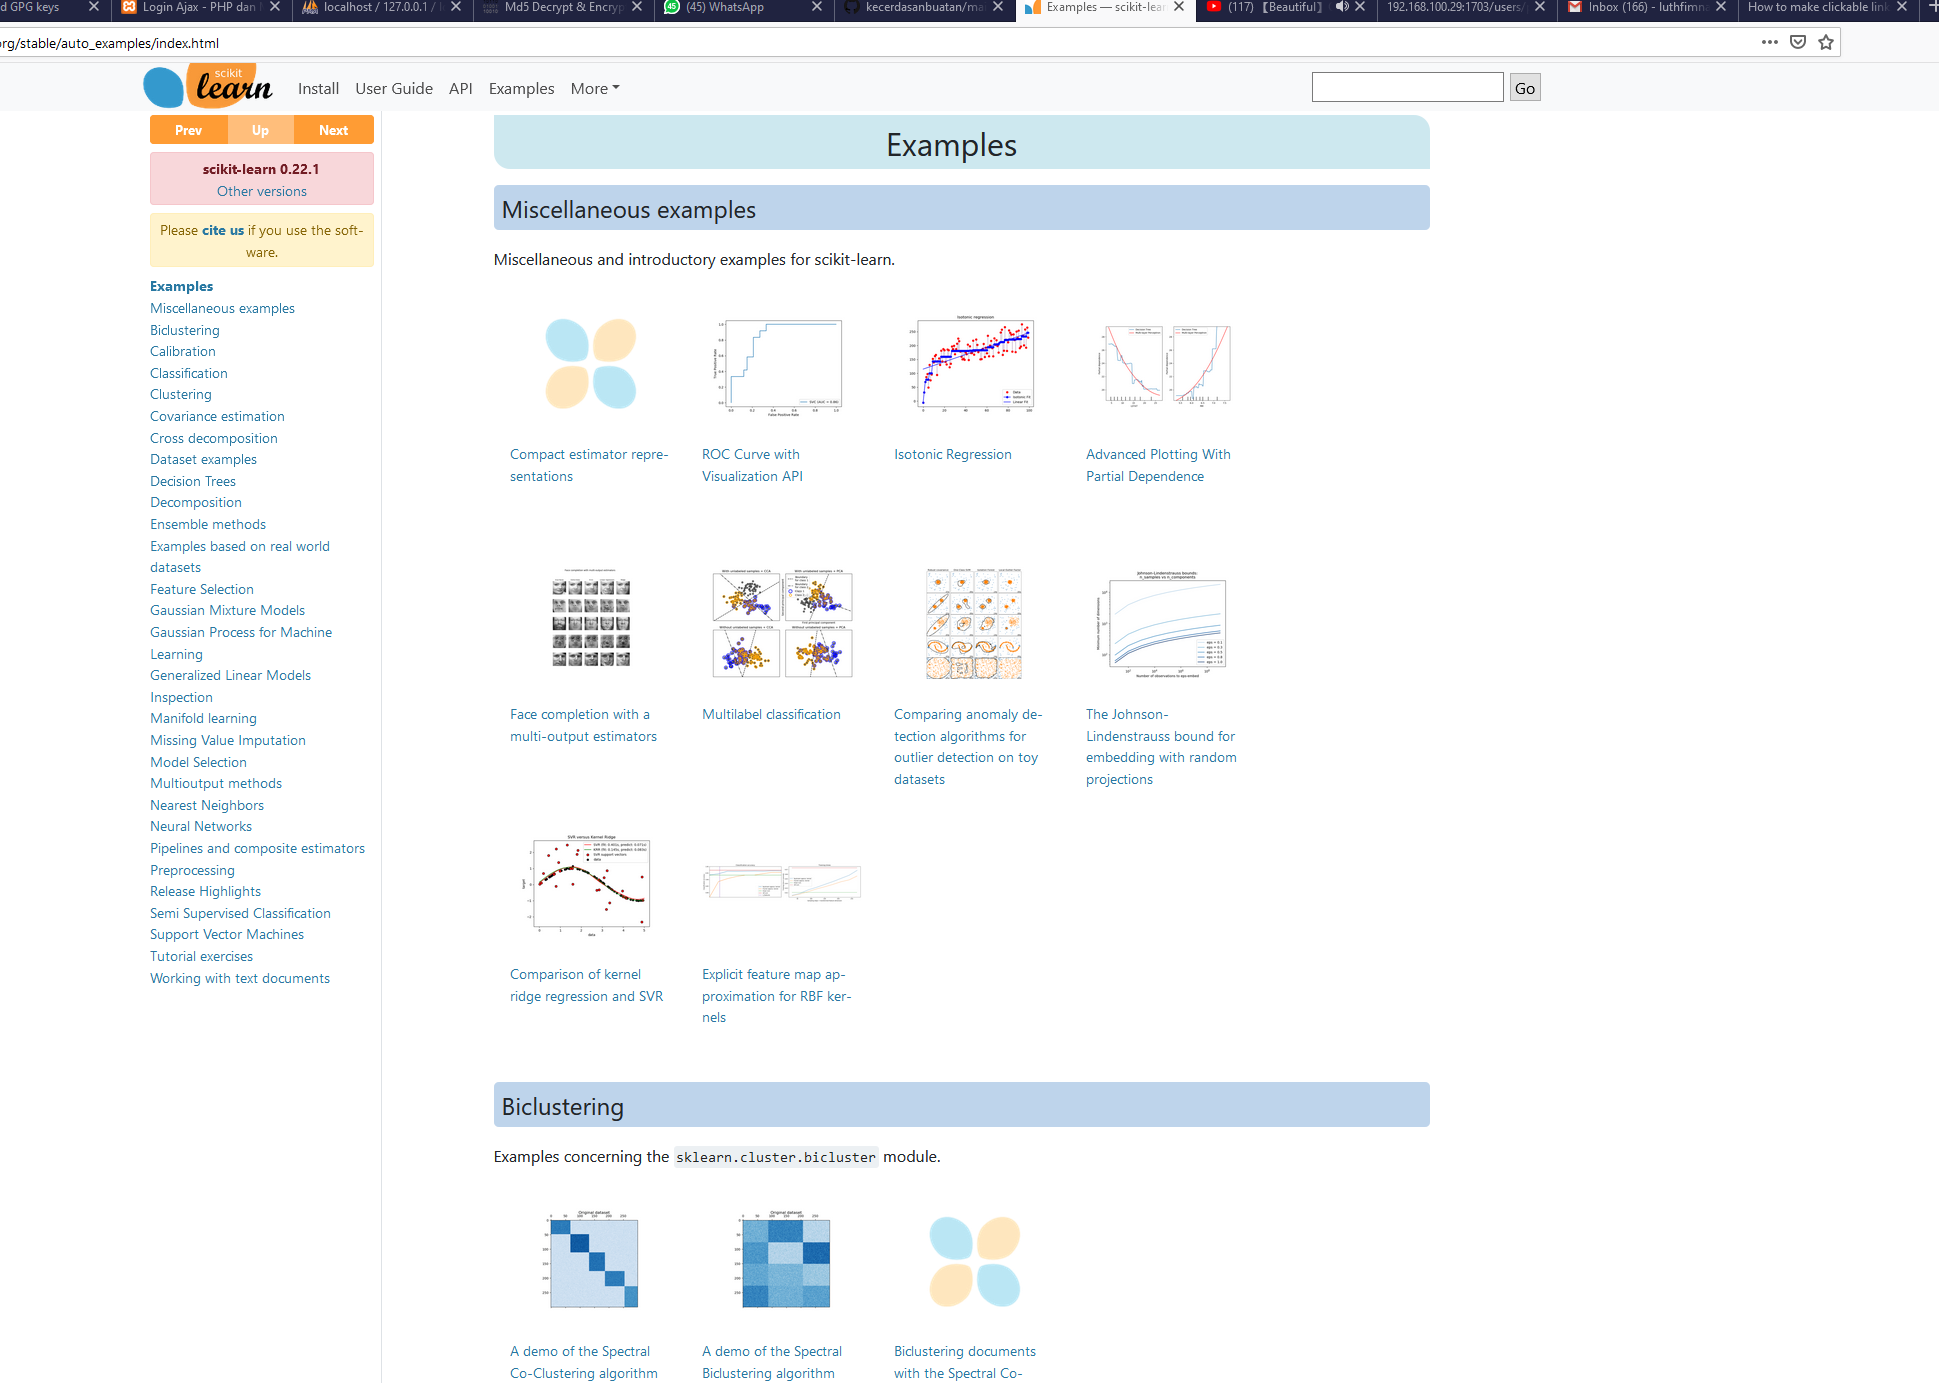
\includegraphics[width=4cm]{figures/1174035/chapter1/1_2.png}
		\centering
		\caption{Daftar Example}
	\end{figure}
	\item Lalu coba jalankan aplikasi tersebut, bisa dicek hasil dari Variable explorernya
	\begin{figure}[H]
		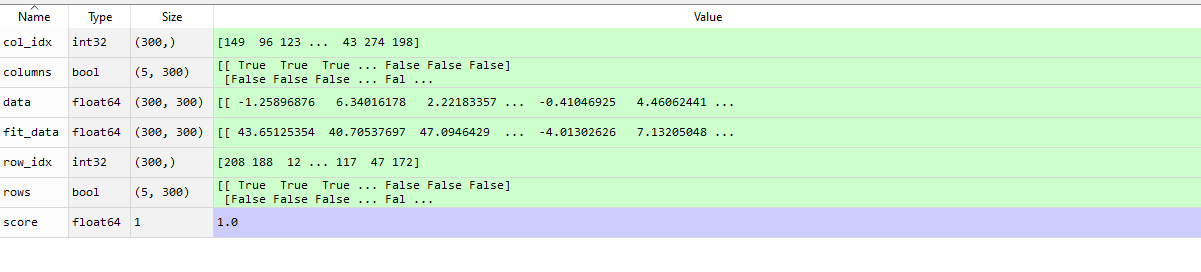
\includegraphics[width=4cm]{figures/1174035/chapter1/1_3.png}
		\centering
		\caption{Variable Explorer}
	\end{figure}
	\item Sample kode \hfill \break \lstinputlisting[firstline=1]{src/1174035/chapter1/sample1.py}
\end{enumerate}

\subsection{Mencoba Loading and example dataset}
Disini akan dilakukan percobaan dengan menggunakan beberapa datasets seperti digits dan iris untuk bisa digunakan sebagai training set yang akan dipakai seluruh metode.
\begin{itemize}
	\item Percobaan 1 (Memuat data iris dan digits dari datasets) \hfill \break \lstinputlisting[firstline=8, lastline=10]{src/1174035/chapter1/sample2.py}
	\begin{figure}[H]
		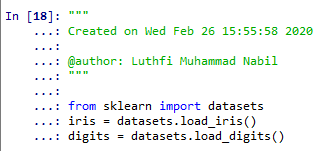
\includegraphics[width=4cm]{figures/1174035/chapter1/2_1_hasil.png}
		\centering
		\caption{Hasil Percobaan 1}
	\end{figure}
	\item Percobaan 2 (Menampilkan data dari digits) \hfill \break \lstinputlisting[firstline=12, lastline=12]{src/1174035/chapter1/sample2.py}
	\begin{figure}[H]
		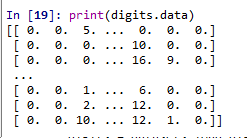
\includegraphics[width=4cm]{figures/1174035/chapter1/2_2_hasil.png}
		\centering
		\caption{Hasil Percobaan 2}
	\end{figure}
	\item Percobaan 3 (Menampilkan digits.target) \hfill \break \lstinputlisting[firstline=14, lastline=14]{src/1174035/chapter1/sample2.py}
	\begin{figure}[H]
		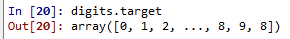
\includegraphics[width=4cm]{figures/1174035/chapter1/2_3_hasil.png}
		\centering
		\caption{Hasil Percobaan 3}
	\end{figure}
	\item Percobaan 4 (Menampilkan data 2 dimensi) \hfill \break \lstinputlisting[firstline=16, lastline=16]{src/1174035/chapter1/sample2.py}
	\begin{figure}[H]
		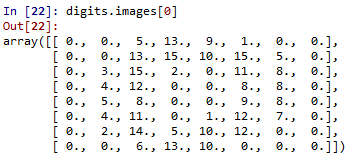
\includegraphics[width=4cm]{figures/1174035/chapter1/2_4_hasil.png}
		\centering
		\caption{Hasil Percobaan 4}
	\end{figure}
	\item Full sample \hfill \break \lstinputlisting[firstline=1]{src/1174035/chapter1/sample2.py}
	\begin{figure}[H]
		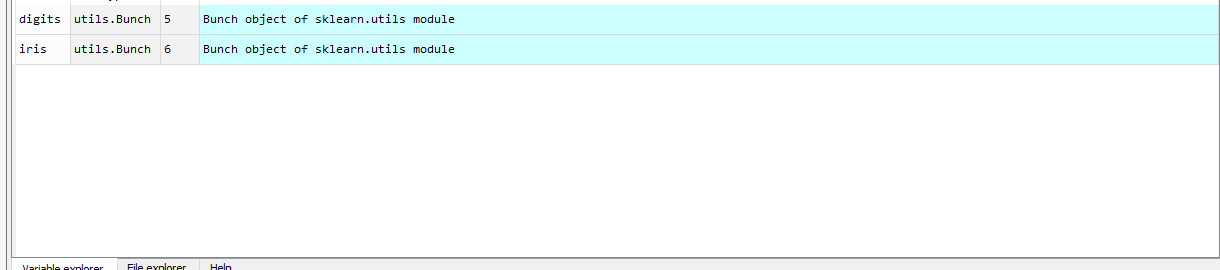
\includegraphics[width=4cm]{figures/1174035/chapter1/2_var.png}
		\centering
		\caption{Hasil pada variable explorer}
	\end{figure}
\end{itemize}
\subsection{Learning and Predicting}
Disini akan dicoba untuk melakukan prediksi berupa angka yang inputnya berupa gambaran dataset. 
\begin{itemize}
	\item Percobaan 1  \hfill \break \lstinputlisting[firstline=8, lastline=11]{src/1174035/chapter1/sample3.py}
	\begin{figure}[H]
		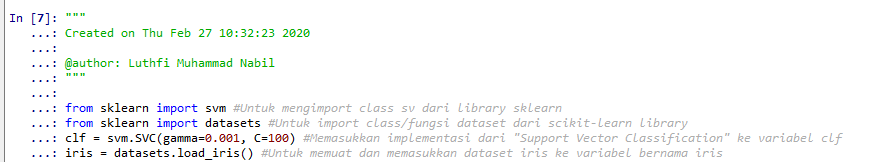
\includegraphics[width=4cm]{figures/1174035/chapter1/3_1_hasil.png}
		\centering
		\caption{Hasil Percobaan 1}
	\end{figure}
	\item Percobaan 2 \hfill \break \lstinputlisting[firstline=13, lastline=14]{src/1174035/chapter1/sample3.py}
	\begin{figure}[H]
		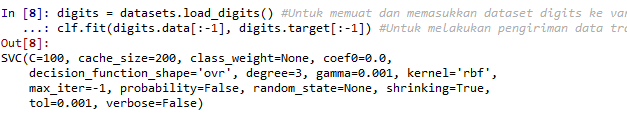
\includegraphics[width=4cm]{figures/1174035/chapter1/3_2_hasil.png}
		\centering
		\caption{Hasil Percobaan 2}
	\end{figure}
	\item Percobaan 3  \hfill \break \lstinputlisting[firstline=16, lastline=16]{src/1174035/chapter1/sample3.py}
	\begin{figure}[H]
		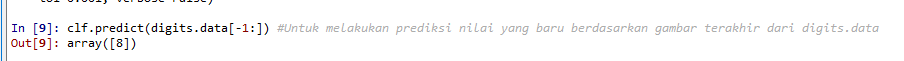
\includegraphics[width=4cm]{figures/1174035/chapter1/3_3_hasil.png}
		\centering
		\caption{Hasil Percobaan 3}
	\end{figure}
	\item Full sample \hfill \break \lstinputlisting[firstline=1]{src/1174035/chapter1/sample3.py}
	\begin{figure}[H]
		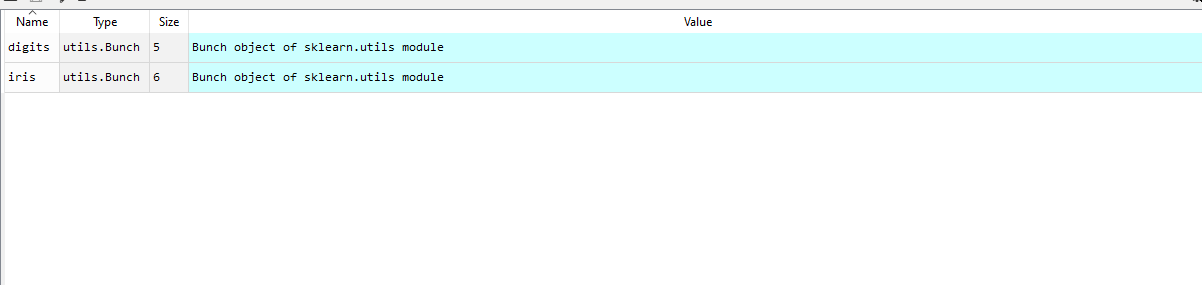
\includegraphics[width=4cm]{figures/1174035/chapter1/3_var.png}
		\centering
		\caption{Hasil pada variable explorer}
	\end{figure}
\end{itemize}
\subsection{Model Persistence}
Disini akan dilakukan persistensi model menggunakan built-in dari Python
\begin{itemize}
	\item Percobaan 1  \hfill \break \lstinputlisting[firstline=8, lastline=12]{src/1174035/chapter1/sample4.py}
	\begin{figure}[H]
		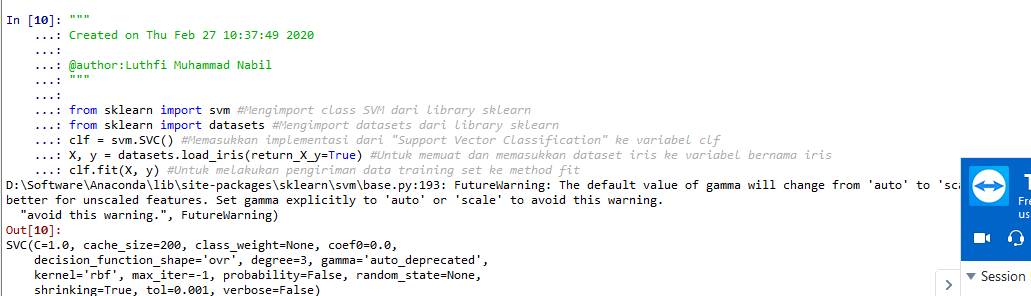
\includegraphics[width=4cm]{figures/1174035/chapter1/4_1_hasil.png}
		\centering
		\caption{Hasil Percobaan 1}
	\end{figure}
	\item Percobaan 2 \hfill \break \lstinputlisting[firstline=14, lastline=17]{src/1174035/chapter1/sample4.py}
	\begin{figure}[H]
		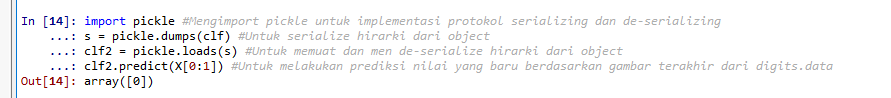
\includegraphics[width=4cm]{figures/1174035/chapter1/4_2_hasil.png}
		\centering
		\caption{Hasil Percobaan 2}
	\end{figure}
	\item Percobaan 3  \hfill \break \lstinputlisting[firstline=19, lastline=19]{src/1174035/chapter1/sample4.py}
	\begin{figure}[H]
		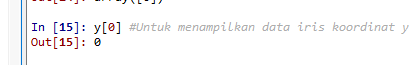
\includegraphics[width=4cm]{figures/1174035/chapter1/4_3_hasil.png}
		\centering
		\caption{Hasil Percobaan 3}
	\end{figure}
	\item Percobaan 4  \hfill \break \lstinputlisting[firstline=21, lastline=22]{src/1174035/chapter1/sample4.py}
	\begin{figure}[H]
		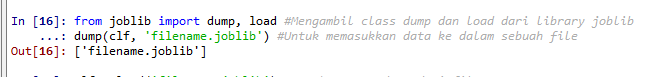
\includegraphics[width=4cm]{figures/1174035/chapter1/4_4_hasil.png}
		\centering
		\caption{Hasil Percobaan 4}
	\end{figure}
	\item Percobaan 5  \hfill \break \lstinputlisting[firstline=24, lastline=24]{src/1174035/chapter1/sample4.py}
	\begin{figure}[H]
		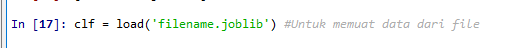
\includegraphics[width=4cm]{figures/1174035/chapter1/4_5_hasil.png}
		\centering
		\caption{Hasil Percobaan 5}
	\end{figure}
	\item Full sample \hfill \break \lstinputlisting[firstline=1]{src/1174035/chapter1/sample4.py}
	\begin{figure}[H]
		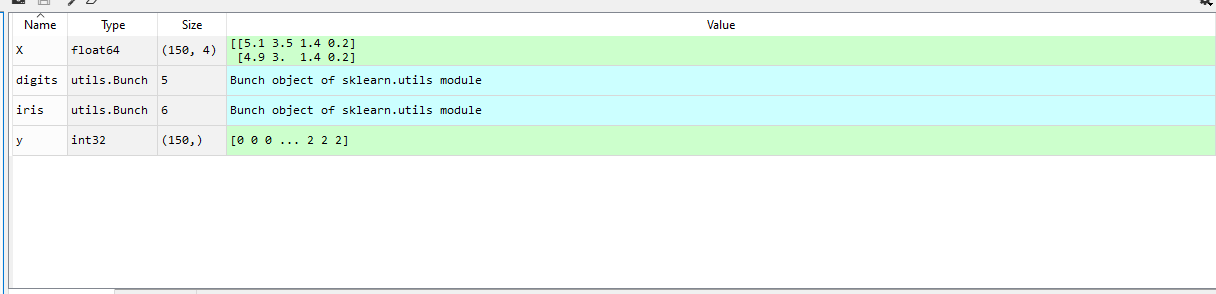
\includegraphics[width=4cm]{figures/1174035/chapter1/4_var.png}
		\centering
		\caption{Hasil pada variable explorer}
	\end{figure}
\end{itemize}
\subsection{Conventions}
Seluruh metode akan dilakukan pengaturan untuk membuat tingkah laku lebih dapat diprediksi
\begin{itemize}
	\item Percobaan 1  \hfill \break \lstinputlisting[firstline=8, lastline=14]{src/1174035/chapter1/sample5.py}
	\begin{figure}[H]
		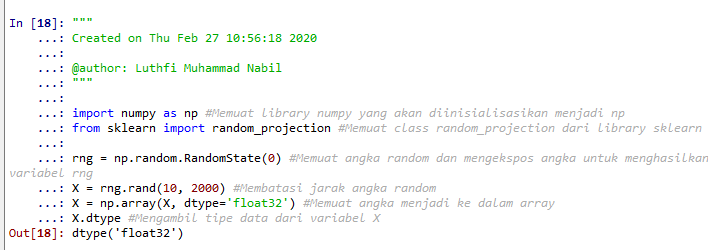
\includegraphics[width=4cm]{figures/1174035/chapter1/5_1_hasil.png}
		\centering
		\caption{Hasil Percobaan 1}
	\end{figure}
	\item Percobaan 2 \hfill \break \lstinputlisting[firstline=16, lastline=18]{src/1174035/chapter1/sample5.py}
	\begin{figure}[H]
		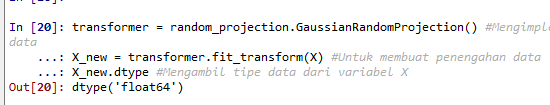
\includegraphics[width=4cm]{figures/1174035/chapter1/5_2_hasil.png}
		\centering
		\caption{Hasil Percobaan 2}
	\end{figure}
	\item Percobaan 3  \hfill \break \lstinputlisting[firstline=21, lastline=25]{src/1174035/chapter1/sample5.py}
	\begin{figure}[H]
		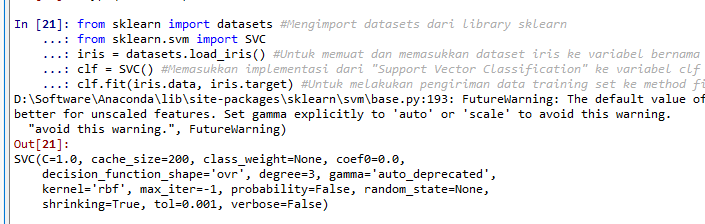
\includegraphics[width=4cm]{figures/1174035/chapter1/5_3_hasil.png}
		\centering
		\caption{Hasil Percobaan 3}
	\end{figure}
	\item Percobaan 4  \hfill \break \lstinputlisting[firstline=27, lastline=27]{src/1174035/chapter1/sample5.py}
	\begin{figure}[H]
		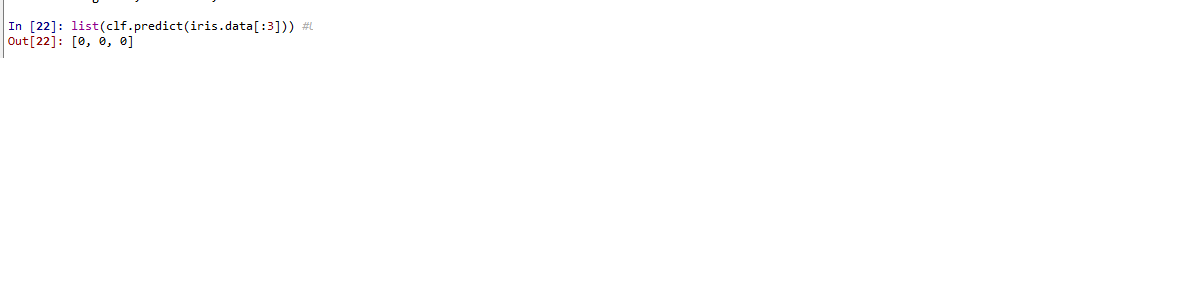
\includegraphics[width=4cm]{figures/1174035/chapter1/5_4_hasil.png}
		\centering
		\caption{Hasil Percobaan 4}
	\end{figure}
	\item Percobaan 5  \hfill \break \lstinputlisting[firstline=29, lastline=29]{src/1174035/chapter1/sample5.py}
	\begin{figure}[H]
		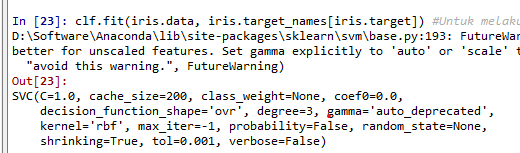
\includegraphics[width=4cm]{figures/1174035/chapter1/5_5_hasil.png}
		\centering
		\caption{Hasil Percobaan 5}
	\end{figure}
	\item Percobaan 6  \hfill \break \lstinputlisting[firstline=31, lastline=31]{src/1174035/chapter1/sample5.py}
	\begin{figure}[H]
		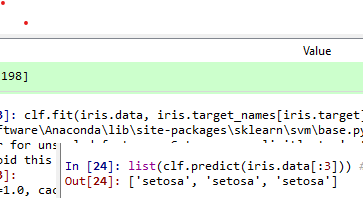
\includegraphics[width=4cm]{figures/1174035/chapter1/5_6_hasil.png}
		\centering
		\caption{Hasil Percobaan 6}
	\end{figure}
	\item Full sample \hfill \break \lstinputlisting[firstline=1]{src/1174035/chapter1/sample5.py}
	\begin{figure}[H]
		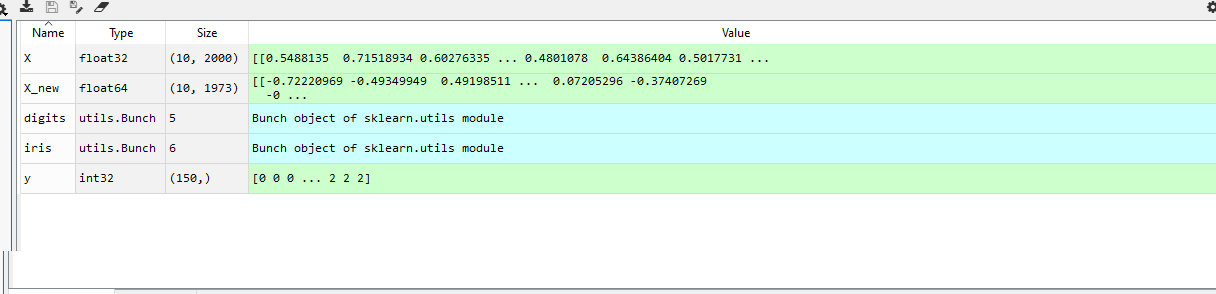
\includegraphics[width=4cm]{figures/1174035/chapter1/5_var.png}
		\centering
		\caption{Hasil pada variable explorer}
	\end{figure}
\end{itemize}
\subsection{Skrinsut Error}
\begin{figure}[H]
	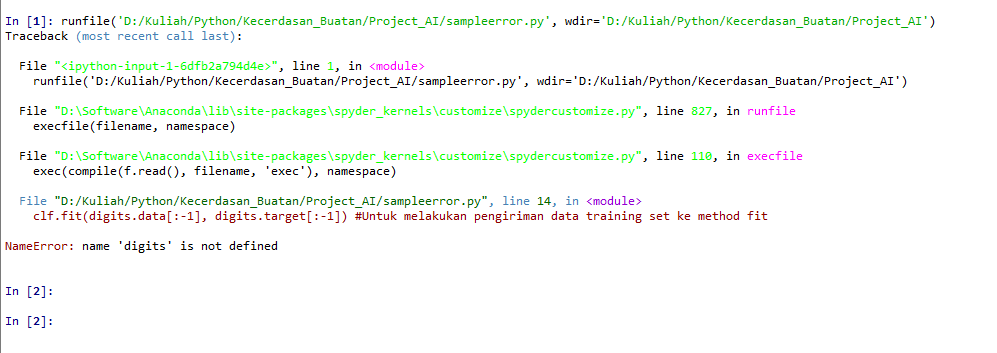
\includegraphics[width=4cm]{figures/1174035/chapter1/skrinsuterror.png}
	\centering
	\caption{Hasil Percobaan 6}
\end{figure}
\subsection{Kode error dan jenis error tersebut}
Error yang didapat berjenis name error, karena sebuah variabel tidak didefinisikan. Yaitu digits
\lstinputlisting[firstline=1]{src/1174035/chapter1/sample5.py}
\subsection{Penanganan Error}
Untuk menangani error tersebut, bisa ditambahkan sesuai instruksi. Yaitu menambahkan sebuah variabel bernama digits. Selain itu, digits harus dapat bekerja sebagaimana mestinya. Berikut full kodingnya : 
\lstinputlisting[firstline=1]{src/1174035/chapter1/sample3.py}
\subsection{Plagiarisme}
\begin{figure}[H]
	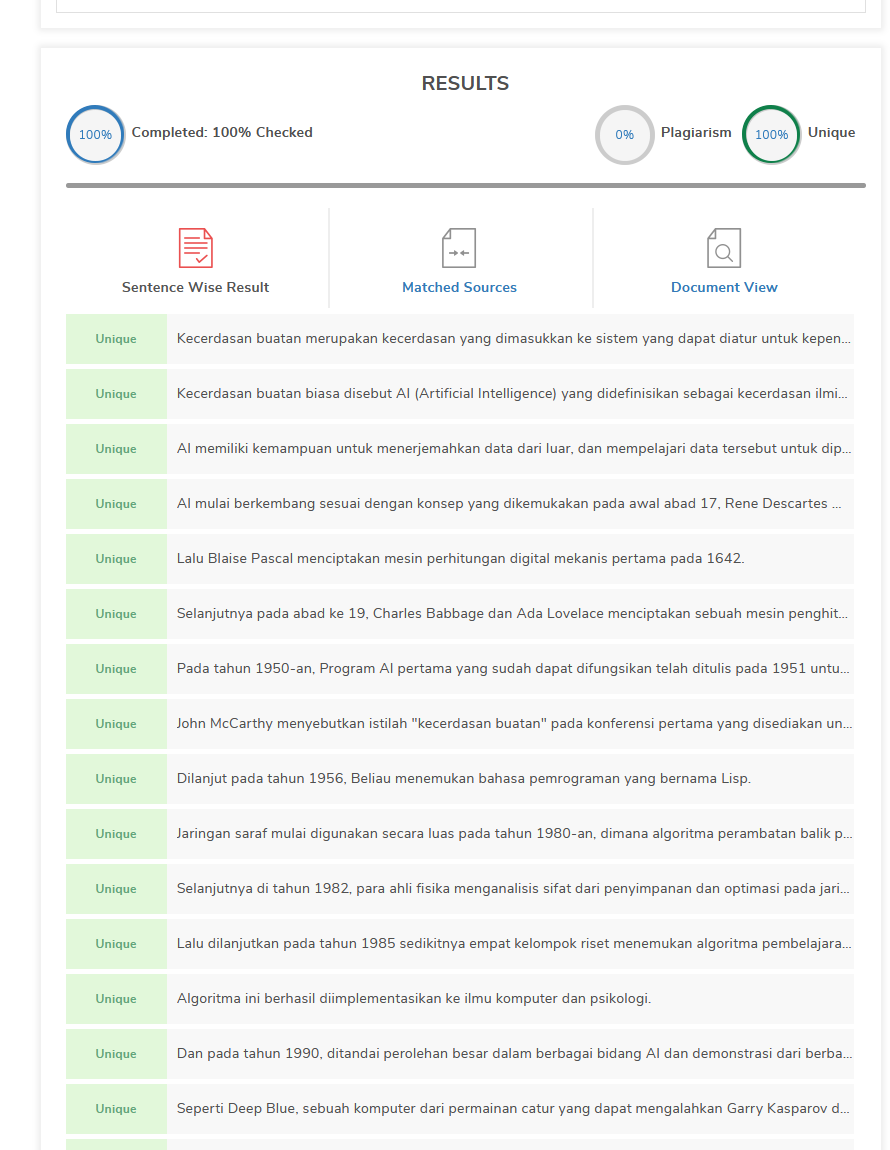
\includegraphics[width=4cm]{figures/1174035/chapter1/plagiarism.png}
	\centering
	\caption{Hasil pada variable explorer}
\end{figure}
\section{1174040 - Hagan Rowlenstino A. S}
    \subsection{Teori}
        \subsubsection{Definisi Kecerdasan Buatan}

        Artificial Inteligence atau dapat disebut juga dengan kecerdasan buatan merupakan kecerdasan yang ditambahakn kepada suatu sistem yang dapat diatur dalam konteks ilmiah.Michael Haenlein dan Andreas Kaplan mendefinisikan bahawa AI adalah “kemampuan sebuah sistem untuk menejerjemahkan data eksternal dengan benar, mempelajari data tersebut, dan menggunakannya guna mencapai tujuan dan tugas tertentu melalui adaptasi yang fleksibel”. Kecerdasan ini dibuat dan dimasukkan ke dalam mesin agar dapat melakukan pekerjaan seperti yang dapat dilakukan manusia dengan cepat dan tepat. Bidang- bidang yang menggunakan kecerdasan buatan antara lain logika fuzzy, permainan komputer (games), sistem pakar, jaringan saraf tiruan dan robotika.
        
        \subsubsection{Sejarah Kecerdasan Buatan}
        
        Sejarah kecerdasan buatan ini dimulai dari zaman kuno, mitos ataupun cerita dan desas-desus tentang sebuah mahkluk yang mempunyai kecerdasan serta kesadaran yang diberikan oleh pengrajin. Benih - benih nya mulai ditanam oleh para filsuf klasik yang mencari cara untuk menggambarkan proses berfikir manusia sebagai manipulasi simbol secara mekanis yang memuncah pada penemuan komputer digital di tahun 1940-an, yaitu sebuah mesin yang didasarkan penalaran matematika. Istilah kecerdasan buatan sendiri baru muncul pada tahun 1956, dan teori -teori nya sudah muncul sejak tahun 1941.

        \subsubsection{Perkembangan Kecerdasan Buatan}
        \begin{enumerate}
            \item Perkembangan kecerdasan buatan dimulai dari Era Komputer Elektronik pada tahun 1941. dimana ditemukannya alat penyimpanan dan pemrosesan informasi. Dilanjutkan pada tahun 1949, berhasilnya pembuatan komputer yang mampu menyimpan program yang memunat pekerjaan dalam memasukkan program menjadi lebih mudah.
            \item Masa - masa persiapan AI terjadi pada tahun 1943 - 1956.
            \item Awal Perkembangan AI terjadi pada 1952 - 1969
            \item Perkembagan kecerdasan buatan melambat pada tahun 1966-1974
            \item Sistem Berbasis Pengetahuan pada tahun 1969-1979
            \item ecerdasan Buatan menjadi sebuah industri pada tahun 1980-1988. Kembalinya Jaringan Syaraf tiruan pada tahun 1986-sekarang.
        \end{enumerate}
    \subsection{Instalasi}
        Membuka  https://scikit-learn.org/stable/tutorial/basic/tutorial.html lalu mencobanya.
        \subsubsection{Instalasi library scikit, mencoba kompilasi dan ujicoba contoh kode}
        \begin{enumerate}
            \item Buka anaconda prompt lalu ketikkan "pip install -U scikit-learn" untuk menginstall library scikit
            \begin{figure}[H]
                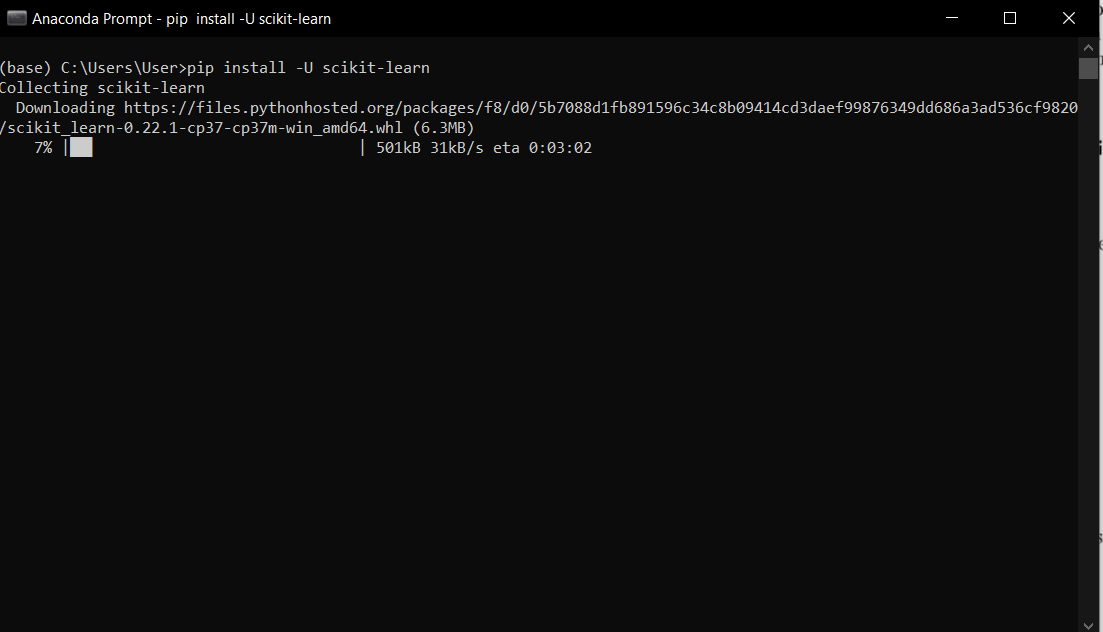
\includegraphics[width=4cm]{figures/1174040/chap1/1.png}
                \centering
                \caption{Install Library Scikit}
            \end{figure}
            \item Pilih salah satu example dari website tersebut lalu jalankan \hfill \break \lstinputlisting[firstline=1]{src/1174040/chap1/ex1.py}
            
            \item buka variable explolernya
            \begin{figure}[H]
                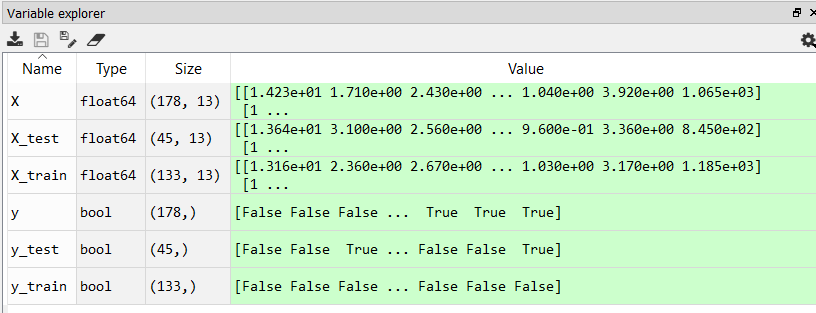
\includegraphics[width=4cm]{figures/1174040/chap1/2.png}
                \centering
                \caption{Variable Exploler}
            \end{figure}
        \end{enumerate}
        \subsubsection{Mencoba loading an example dataset}
        \begin{enumerate}
            \item mengambil data iris dan digit dari dataset \hfill \break \lstinputlisting[firstline=9, lastline=11]{src/1174040/chap1/ex2.py}
            
            \item Menampilkan data digits \hfill \break \lstinputlisting[firstline=13, lastline=13]{src/1174040/chap1/ex2.py}
            
            \begin{figure}[H]
                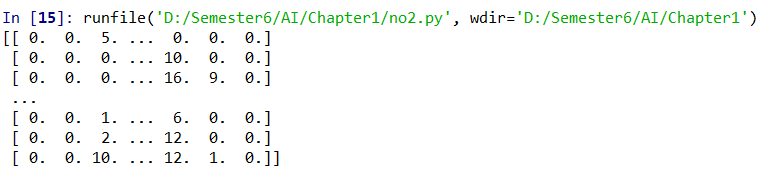
\includegraphics[width=4cm]{figures/1174040/chap1/3.png}
                \centering
                \caption{Data Digits}
            \end{figure}

            \item menampilkan digits.target
            \hfill \break \lstinputlisting[firstline=15, lastline=15]{src/1174040/chap1/ex2.py}

            \begin{figure}[H]
                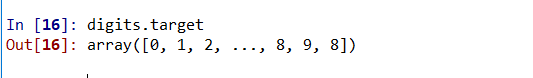
\includegraphics[width=4cm]{figures/1174040/chap1/4.png}
                \centering
                \caption{Digits Target}
            \end{figure}

            \item menampilkan data bentuk 2D. \hfill \break \lstinputlisting[firstline=17, lastline=17]{src/1174040/chap1/ex2.py}

            \begin{figure}[H]
                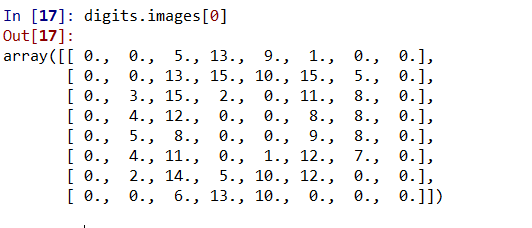
\includegraphics[width=4cm]{figures/1174040/chap1/5.png}
                \centering
                \caption{Data 2D}
            \end{figure}
        \end{enumerate}
\section{1174042 Faisal Najib Abdullah}
\subsection{Teori}
\begin{enumerate}
\item Definisi, sejarah, dan perkembangan kecerdasan buatan.
\subitem Definisi kecerdasan buatan adalah suatu pengetahuan yang dapat membuat komputer untuk meniru kecerdasan manusia yang berhubungan dengan penangkapan, pemodelan, dan penyimpanan kecerdasan manusia dalam sebuah sistem teknologi. Contohnya yaitu melakukan analisa penalaran untuk mengambil suatu kesimpulan atau penerjemahan atau keputusan dari satu bahasa satu ke bahasa lain.
\subitem Sejarah dan perkembangan kecerdasan buatan terjadi pada musim panas tahun 1956 tercatat adanya seminar mengenai AI di Darmouth College. Seminar pada waktu itu dihadiri oleh sejumlah pakar komputer dan membahas potensi komputer dalam meniru kepandaian manusia. Akan tetapi perkembangan yang sering terjadi semenjak diciptakannya LISP, yaitu bahasa kecerdasan buatan yang dibuat tahun 1960 oleh John McCarthy. Istilah pada kecerdasan buatan atau Artificial Intelligence diambil dari Marvin Minsky dari MIT. Dia menulis karya ilmiah berjudul Step towards Artificial Intelligence, The Institute of radio Engineers Proceedings 49, January 1961\cite{baraja2008kecerdasan}. 
\item  Definisi supervised learning, klasifikasi, regresi, dan unsupervised learning. Data set, training set dan testing set. 
\subitem Supervised learning merupakan sebuah pendekatan dimana sudah terdapat data yang dilatih, dan terdapat variable yang ditargetkan sehingga tujuan dari pendekatan ini adalah mengkelompokan suatu data ke data yang sudah ada. Sedangkan unsupervised learning tidak memiliki data latih, sehingga dari data yang ada, kita mengelompokan data tersebut menjadi 2 bagian atau 3 bagian dan seterusnya.
\subitem Klasifikasi adalah salah satu topik utama dalam data mining atau machine learning. Klasifikasi yaitu suatu pengelompokan data dimana data yang digunakan tersebut mempunyai kelas label atau target.
\subitem Regresi adalah Supervised learning tidak hanya mempelajari classifier, tetapi juga mempelajari fungsi yang dapat memprediksi suatu nilai numerik. Contoh, ketika diberi foto seseorang, kita ingin memprediksi umur, tinggi, dan berat orang yang ada pada foto tersebut.
\subitem Data set adalah cabang aplikasi dari Artificial Intelligence/Kecerdasan Buatan yang fokus pada pengembangan sebuah sistem yang mampu belajar sendiri tanpa harus berulang kali di program oleh manusia.
\subitem Training set yaitu jika pasangan objek, dan kelas yang menunjuk pada objek tersebut adalah suatu contoh yang telah diberi label akan menghasilkan suatu algoritma pembelajaran.
\subitem Testing set digunakan untuk mengukur sejauh mana classifier berhasil melakukan klasifikasi dengan benar\cite{zhu2009introduction}.
\end{enumerate}

\subsection{Instalasi}
\subsubsection{Instalasi Library Scikit dari Pycharm}
Masuk pada menu settings terus pilih Project Interpreter kemudian tambah library lalu cari dan install scikit
\begin{figure}[ht]
\centering
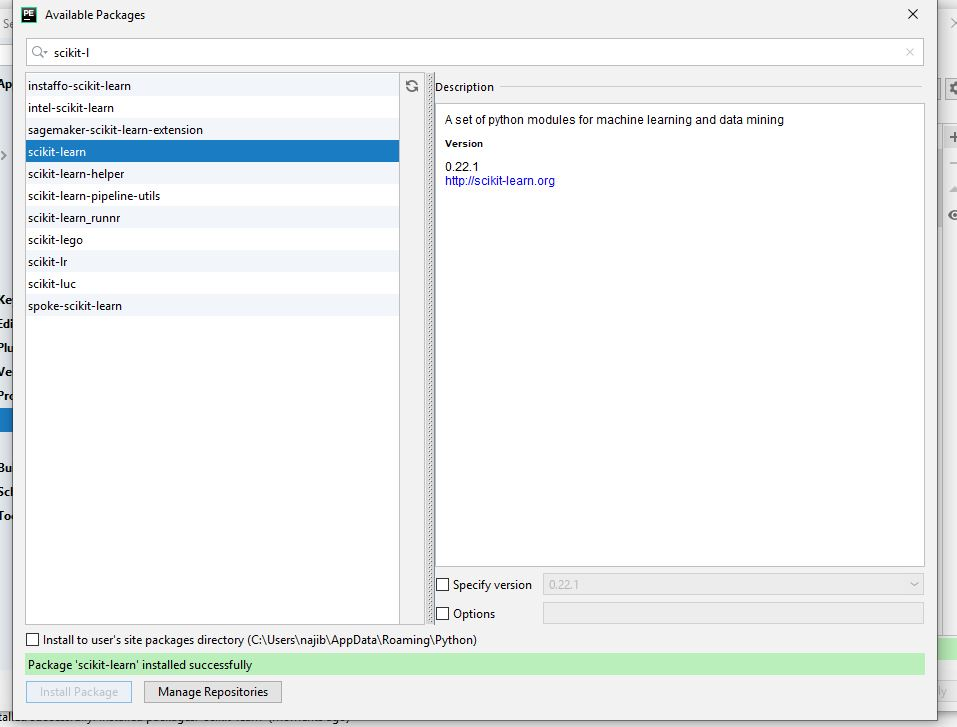
\includegraphics[scale=0.5]{figures/1174042/chapter1/2.jpg}
\caption{Installasi}
\label{contoh}
\end{figure}

Mencoba Library
\lstinputlisting{src/1174042/chapter1/2,1.py}

\subsubsection{Mencoba Loading an example Dataset}
\lstinputlisting{src/1174042/chapter1/2,2.py}
\begin{figure}[ht]
\centering
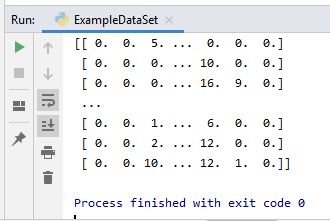
\includegraphics[scale=0.5]{figures/1174042/chapter1/3.jpg}
\caption{Mencoba Loading an example Dataset}
\label{contoh}
\end{figure}

\subsubsection{Learning and Predicting}
\lstinputlisting{src/1174042/chapter1/2,3.py}
\begin{figure}[ht]
\centering
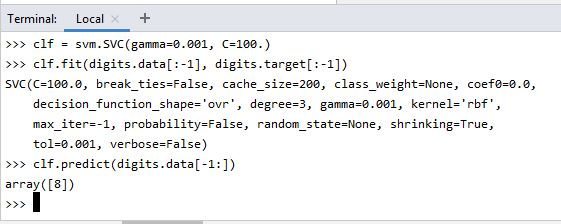
\includegraphics[scale=0.5]{figures/1174042/chapter1/2,3.jpg}
\caption{Learning and Predicting}
\label{contoh}
\end{figure}

\subsubsection{Model Presistence}
\lstinputlisting{src/1174042/chapter1/2,4.py}
\begin{figure}[ht]
\centering
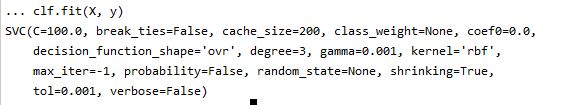
\includegraphics[scale=0.5]{figures/1174042/chapter1/2,4.jpg}
\caption{Model Presistence}
\label{contoh}
\end{figure}

\begin{figure}[ht]
\centering
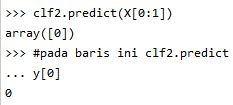
\includegraphics[scale=0.5]{figures/1174042/chapter1/2,4,1.jpg}
\caption{Model Presistence}
\label{contoh}
\end{figure}

\begin{figure}[ht]
\centering
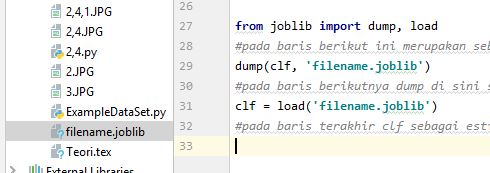
\includegraphics[scale=0.5]{figures/1174042/chapter1/2,4,2.jpg}
\caption{Model Presistence}
\label{contoh}
\end{figure}

\subsubsection{Conventions}
\lstinputlisting{src/1174042/chapter1/2,5.py}


\subsection{Penanganan eror}
\subsubsection{ScreenShoot Eror}
\begin{figure}[ht]
\centering
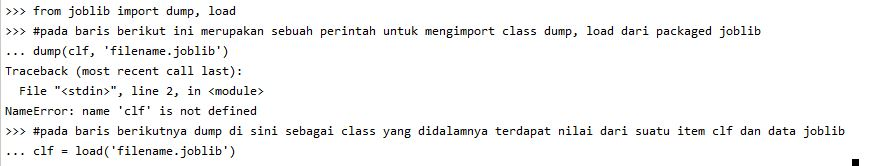
\includegraphics[scale=0.5]{figures/1174042/chapter1/3,1.jpg}
\caption{Error}
\label{contoh}
\end{figure}

\subsubsection{Tuliskan Kode Eror dan Jenis Erornya}
\begin{verbatim}
File "<stdin>", line 2, in <module>
NameError: name 'clf' is not defined
\end{verbatim}


\subsubsection{Solusi Pemecahan Masalah Error}
Ini karna kode di jalankan perbaris perbaris, jika kode dijanlankan bersamaan makan kode berjan sesuai prosedur.

\subsection{Plagiat}
\begin{figure}[ht]
\centering
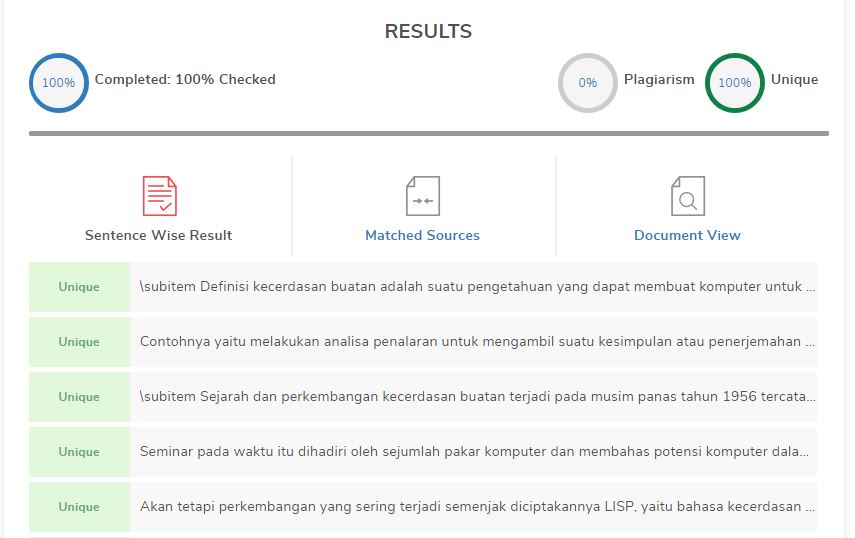
\includegraphics[scale=0.5]{figures/1174042/chapter1/5.jpg}
\caption{Error}
\label{contoh}
\end{figure}
\section{1174043 - Irvan Rizkiansyah}
	\subsection {Definisi Kecerdasan Buatan}
	Kecerdasan buatan atau biasa disebut AI (Artificial Intelligence) merupakan kecerdasan yang dibuat dan ditambahkan oleh manusia ke suatu sistem teknologi, yang diatur dan dikembangkan dalam konteks ilmiah, yang merupakan bentukan dari kecerdasan entitas ilmiah yang ada. Jadi pada intinya definisi AI dapat terus dikembangkan, namun yang menjadi poin utamanya adalah bagaimana manusia menciptakan sebuah teknologi yang dapat berpikir seperti selayaknya manusia itu sendiri.
	
	\subsection{Sejarah dan Perkembangan}
	\begin{itemize}
		\item Program kecerdasan buatan atau Artificial Intelligence pertama kali dicetuskan pada kisaran tahun 1951. Tidak bisa dipungkiri bahwa di tahun tersebut memang sedang gencar-gencarnya pembuatan cikal bakal, konsep, hingga teknologi berbasis AI. Dan, AI sendiri pertama kali digunakan di University of Manchester untuk menjalankan sebuah mesin bernama Ferranti Mark 1.
		\item Beberapa waktu kemudian, Christopher Strachey melanjutkan konsep kecerdasan buatan untuk menjalankan sebuah permainan catur, dimana bidak catur tersebut dapat berjalan secara otomatis dan mampu bermain melawan manusia sungguhan.
		\item Berlanjut pada tahun 1956, kecerdasan buatan tidak hanya dibuat untuk memudahkan bermain catur saja. Melainkan pada saat konferensi pertamanya, John McCharty menamai algoritma teknologi tersebut dengan sebutan “Artificial Intelligence”. Istilah tersebut masih digunakan hingga sekarang oleh para pakar teknologi.
		\item Terakhir, konsep dan teknologi kecerdasan buatan disempurnakan oleh seorang ahli yang namanya masih diingat sampai sekarang sebagai seorang pakar kecerdasan buatan, yaitu Alan Turin. Pada saat itu, Alan Turin meneliti dan menguji coba algoritma AI yang diberi nama dengan “Turing Test”. Hingga seiring berkembangnya waktu, konsep teknologi AI banyak digunakan di berbagai teknologi baik itu multimedia, search engine, dan masih banyak lainnya.
	\end{itemize}
	
	\subsection{Supervised Learning}
	Supervised learning (Pembelajaran terawasi), dalam konteks kecerdasan buatan (AI) dan Machine Learning, adalah jenis sistem di mana input dan output data yang diinginkan disediakan. Input dan output data diberi label untuk klasifikasi untuk memberikan dasar pembelajaran untuk pemrosesan data di masa depan.
	
	\subsection{Unsupervised Learning}
	Unsupervised learning merupakan pembelajan yang tidak terawasi dimana tidak memerlukan target output. Pada metode ini tidak dapat ditentukan hasil seperti apa yang diharapkan selama proses pembelajaran, nilai bobot yang disusun dalam proses range tertentu tergantung pada nilai output yang diberikan. Tujuan metode uinsupervised learning ini agar kita dapat mengelompokkan unit-unit yang hampir sama dalam satu area tertentu.
	
	\subsection{Teknik Klasifikasi}
	Teknik klasifikasi memprediksi respons diskrit, misalnya seperti apakah email itu asli atau spam, atau apakah tumor itu kanker atau tidak. Model klasifikasi mengklasifikasikan data masukan ke dalam kategori tersebut.
	
	\subsection{Regresi}
	Regresi yaitu pengeluaran nilai output yang konstan jika dipicu dengan parameter tertentu biasanya regresi disini berbentuk regresi linier. Regresi linier yaitu metode statistika yang digunakan untuk membentuk model hubungan antara variabel terikat(dependen,respon,Y) dengan satu atau lebih variabel bebas(independent, prdiktor, X). Apabila banyaknya variabel bebas hanya ada satu, disebut sebagai regresi linier sederhana, sedangkan apabila terdapat lebih dari satu variabel bebas, disebut sebagai regresi linier berganda.
	
	\subsection{Training Set}
	Training set adalah bagian dari dataset itu sendiri yang dilatih untuk membuat prediksi atau algoritma mesin learning lainnya sesuai keinginan atau tujuan data itu dibuat.
	
	\subsection{Testing Set}
	Testing set adalah bagian dari dataset yang di tes atau diujicoba untuk melihat keakuratannya dengan katalain melihat peformanya.
	
	\subsection{Instalasi dan Percobaan Kompilasi dari Library Scikit-learn}
	\begin{enumerate}
		\item Buka anaconda prompt
		\item kemudian Ketik di anaconda prompt yaitu : "pip install -U scikit-learn" \break
		\begin{figure}[H]
			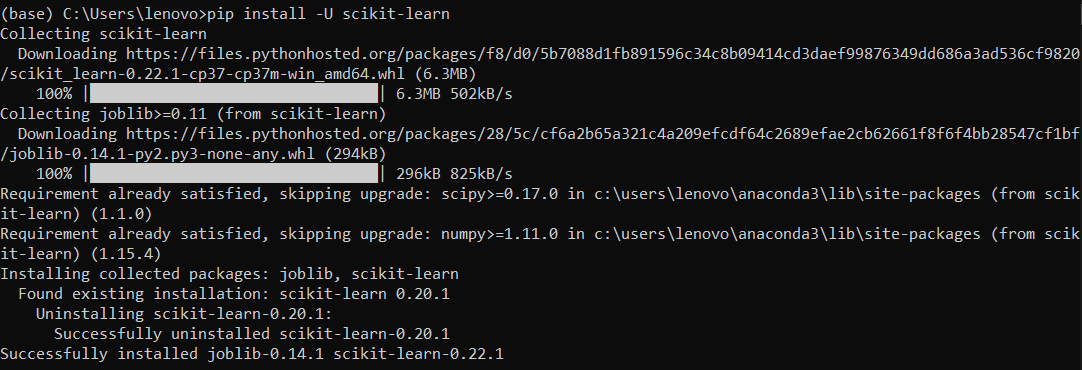
\includegraphics[width=4cm]{figures/1174043/chapter1/1.png}
			\centering
			\caption{Instalasi Scikit Learn}
		\end{figure}
		\item Setelah selesai instalasi, pilih salah satu example dari website Scikit
		\item Sample kode \break \lstinputlisting[firstline=1]{src/1174043/chapter1/sample1.py}
		\item Kemudian jalankan aplikasi tersebut, dan bisa dicek hasil dari Variable explorernya \break
		\begin{figure}[H]
			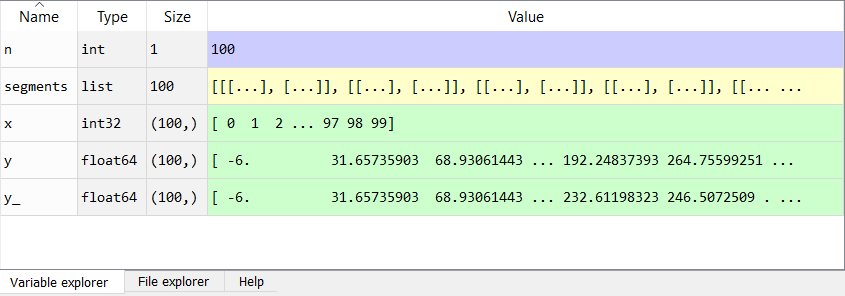
\includegraphics[width=4cm]{figures/1174043/chapter1/hasil_sample.png}
			\centering
			\caption{Variable Explorer}
		\end{figure}
	\end{enumerate}
	
	\subsection{Mencoba Loading an example dataset}
	\begin{enumerate}
		\item Sample kode \break \lstinputlisting[firstline=1]{src/1174043/chapter1/sample2.py}
		\item Kemudian jalankan aplikasi tersebut \break
		\begin{figure}[H]
			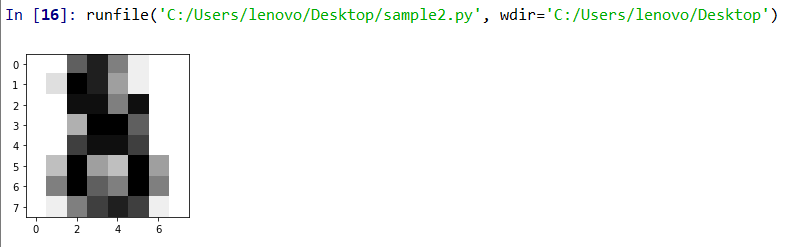
\includegraphics[width=4cm]{figures/1174043/chapter1/hasil_dataset.png}
			\centering
			\caption{Dataset}
		\end{figure}
	\end{enumerate}
\section{1174050 Dika Sukma Pradana}
\subsection{Teori}
\begin{enumerate}
\item Definisi, sejarah, dan perkembangan kecerdasan buatan.
\subitem Intelegensi buatan (AI) mengacu pada simulasi kecerdasan manusia dalam mesin yang diprogram untuk berpikir seperti manusia dan meniru tindakan mereka. Istilah ini juga dapat diterapkan pada mesin apa pun yang menunjukkan sifat-sifat yang terkait dengan pikiran manusia seperti pembelajaran dan pemecahan masalah.
\subitem Sejarah Kecerdasan Buatan (AI) bermula pada saat zaman kuno, dengan sejuta mitos, cerita dan desas-desus tentang makhluk buatan yang diberkahii dengan kecerdasan oleh pengrajin ahli. Benih-benih AI modern ditanam oleh para filsuf klasik yang mencoba menggambarkan proses pemikiran manusia sebagai manipulasi simbol secara mekanis. Karya ini memuncak dalam penemuan komputer digital yang dapat diprogram pada tahun 1940-an, sebuah mesin yang didasarkan pada esensi abstrak penalaran matematika. Perangkat ini dan ide-ide di belakangnya menginspirasi segelintir ilmuwan untuk mulai serius membahas kemungkinan membangun otak elektronik.
Bidang penelitian AI didirikan pada lokakarya yang diadakan di kampus Dartmouth College selama musim panas 1956. Mereka yang hadir akan menjadi pemimpin penelitian AI selama beberapa dekade. Banyak dari merekka meramaIkan bahwa sebuah mesin yang secerdas manusia akan hidup tidak lebih dari satu generasi dan mereka diberi jutaan dolar untuk mewujudkan visi atau tujuan ini.
Akhirnya, menjadi jelas bahwa mereka meremehkan kesulitan proyek. Pada tahun 1973, sebagai tanggapan atas kritik dari James Lighthill dan tekanan terus-menerus dari kongres, AS dan Pemerintah Inggris menghentikan pendanaan penelitian yang tidak diarahkan pada kecerdasan buatan, dan tahun-tahun sulit berikutnya akan dikenal sebagai musim dingin AI. Tujuh tahun kemudian, sebuah inisiatif visioner oleh Pemerintah Jepang mengilhami pemerintah dan industri untuk menyediakan miliaran dolar dalam AI, tetapi pada akhir 80-an investor menjadi kecewa dengan kurangnya daya komputer (perangkat keras) yang dibutuhkan dan menarik lebih banyak dana.
Investasi dan minat pada AI tumbuh pesat pada dekade pertama abad ke-21, ketika pembelajaran mesin berhasil diterapkan pada banyak masalah di dunia akademis dan industri karena metode baru, penerapan perangkat keras komputer yang kuat, dan kumpulan data yang sangat besar.
\item  Definisi supervised learning, klasifikasi, regresi, dan unsupervised learning. Data set, training set dan testing set. 
\subitem Supervised learning adalah sebuah metode pendekatan yang mana sudah terdapat data yang dilatiih, dan terdapat variabel yang ditargetkan atau yang menjadi tujuan sehingga tujuan dari pendekatan ini adalah mengkelompokan suatu data ke data yang sudah ada. Sedangkan unsupervised learrning tidak memiliki data latiih, sehinggga dari data yang ada, kita mengelompokan data tersebbut menjadi dua bagian atau bahkan tiga bagian dan seterusnya.
\subitem Klasifikasi adalah salah satu topik utama dalam data mining atau machine learning. Klasifikasi yaitu suatu pengelompokan data dimana data yang digunakan tersebut mempunyai kelas label atau target.
\subitem Regresi adalah Supervised learning tidak hanya mempelajari classifier, tetapi juga mempelajari fungsi yang dapat memprediksi suatu nilai numerik. 
\subitem Data set merupakan sebuah cabang aplikasi dari Artificial Intelligence(AI)/Kecerdasan Buatan yang terfokus kepada pengembangan sebuah sistem yang mampu belajar sendiiri tannpa harus berulang kalai di program oleh manusia(programmer).
\subitem Training set yaitu jika pasangan objek, dan kelas yang menunjuk pada objek tersebut adalah suatu contoh yang telah diberi label akan menghasilkan suatu algoritma pembelajaran.
\subitem Testing set digunakan untuk mengukur sejauh mana classifier berhasil melakukan klasifikasi dengan benar\cite{zhu2009introduction}.
\end{enumerate}

\subsection{Instalasi}
\subsubsection{Instalasi Library Scikit dari Anaconda}
\begin{enumerate}
\item Download aplikasi Anaconda terlebih dahulu. 
\item Install aplikasi Anaconda yang sudah di download tadi. 
\item Simpan aplikasi sesuai folder yang kita pilih lalu next. 
\item Centang Keduanya lalu tekan tombol install. 
\item Setelah itu tunggu sampai proses instalasi selesai lalu jika sudah tekan tombol finish. 
\item Lalu buka command prompt anda dan tuliskan perintah berikut ini untuk mengecek apakah aplikasinya sudah terinstall. 
\item Kemudian ketikkan perinta pip install -U scikit-learn seperti gambar berikut. 
\end{enumerate}
         \begin{figure}[H]
                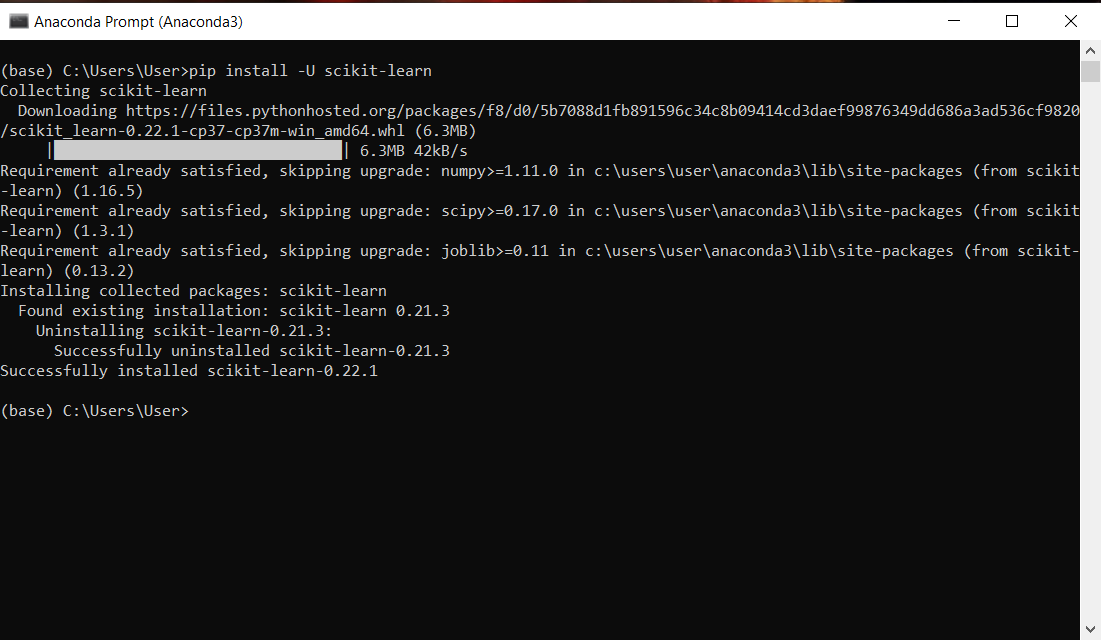
\includegraphics[width=4cm]{figures/1174050/chapter1/instal.png}
                \centering
                \caption{Instalasi}
            \end{figure}


\subsection{Percobaan}
Mencoba Library
\lstinputlisting{src/1174050/chapter1/VAR.py}
 \begin{figure}[H]
                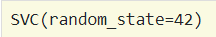
\includegraphics[width=4cm]{figures/1174050/chapter1/2.png}
                \centering
                \caption{Variabel Explore}
            \end{figure}


\subsubsection{Mencoba Loading an example Dataset}
\lstinputlisting{src/1174050/chapter1/dataset.py}
 \begin{figure}[H]
                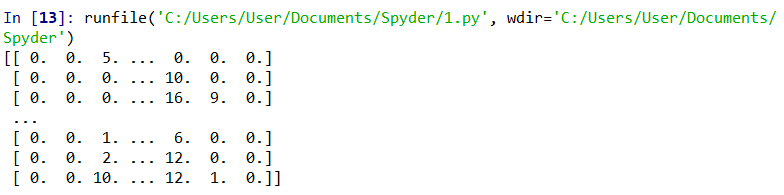
\includegraphics[width=4cm]{figures/1174050/chapter1/1.png}
                \centering
                \caption{Datasets}
            \end{figure}


\subsubsection{Learning and Predicting}
\lstinputlisting{src/1174050/chapter1/learning.py}


\subsubsection{Model Presistence}
\lstinputlisting{src/1174050/chapter1/modelpersistance.py}


\subsubsection{Conventions}
Type Casting
\lstinputlisting{src/1174050/chapter1/typecasting.py}
Refitting and updating parameters
\lstinputlisting{src/1174050/chapter1/Multiclass.py}
Multiclass vs. multilabel fitting
\lstinputlisting{src/1174050/chapter1/Refitting.py}


\subsection{Penanganan eror}
\subsubsection{ScreenShoot Eror}
\begin{figure}[ht]
\centering
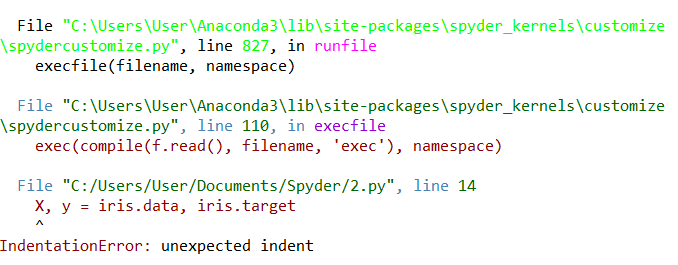
\includegraphics[scale=0.5]{figures/1174050/chapter1/error.png}
\caption{Error}
\label{contoh}
\end{figure}

\subsubsection{Tuliskan Kode Eror dan Jenis Erornya}
\begin{verbatim}
IndentationError: unexpected indent
\end{verbatim}


\subsubsection{Solusi Pemecahan Masalah Error}
Pastikan semua spasi pada koding sama. Menggunakan spasi atau tab.

\subsection{Plagiarism}
\begin{figure}[ht]
\centering
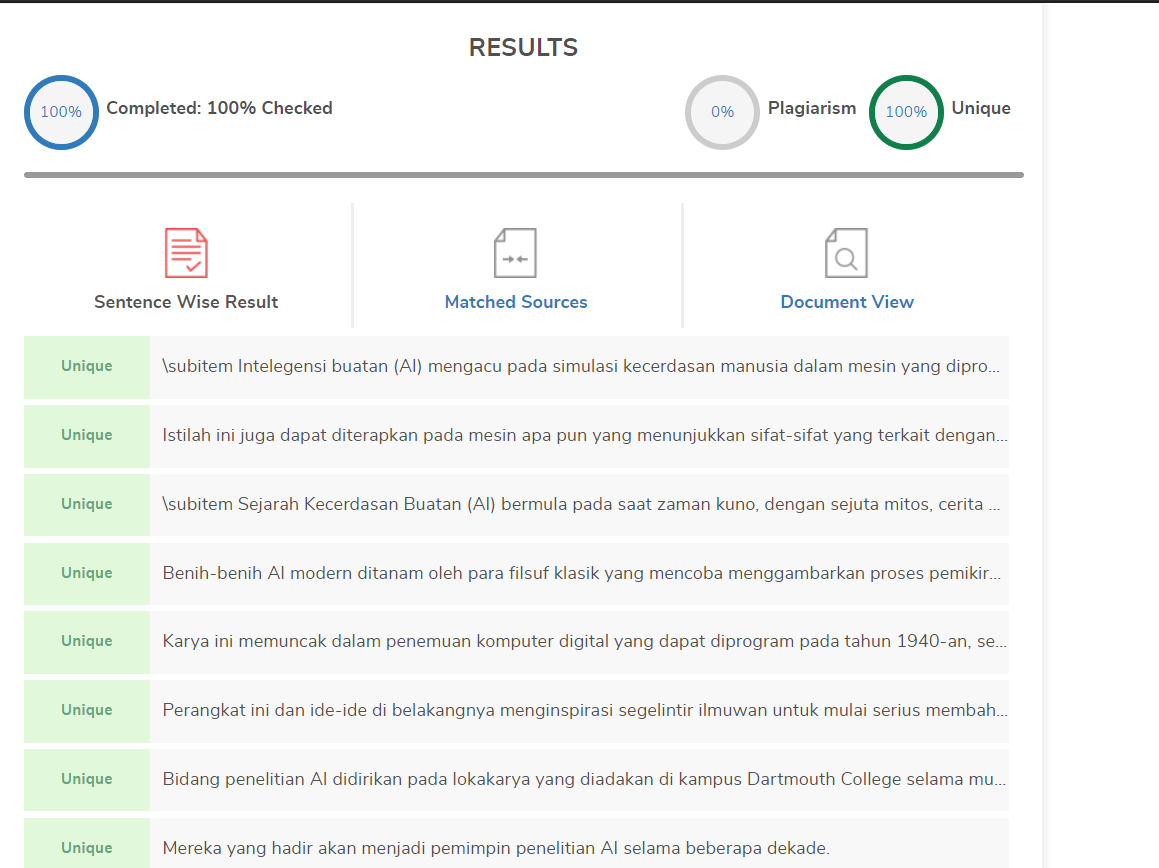
\includegraphics[scale=0.5]{figures/1174050/chapter1/plagiarism.png}
\caption{Plagiarism}
\end{figure}
\section{1174057 Alit Fajar Kurniawan}
\subsection{Teori}
	\subsubsection {Sejarah Perkembangan dan Definisi Artificial Intelligence}
	\par Kecerdasan buatan merupakan sebuah bidang dalam ilmu computer yang begitu penting di zaman ini dan masa yang akan datang guna mewujudkan sebuah sistem computer yang begitu cerdas. Artificial Intelligence atau biasa di singkat dengan AI berasal dari bahasa latin yang dimana intelligence berarti saya paham.
	\par Pada tahun 1955, Newell dan juga Simon telah mengembangkan The Logic Theorist, yaitu program AI pertama. Dimana program tersebut mempresentasikan sebuah masalah sebagai model pohon, lalu diselesaikan dengaan cara memilih cabang yang akan mewujudkan kesimpulan terbenar dan tepat. Program AI tersebut berdampak sangat besar dan dapat mendaji batu loncatan yang cukup penting dalam mengembangkan bidang AI \cite{baraja2008kecerdasan}.
	\par
	Masa Perkembangan AI dimulai pada awal era komputer elektronik pada tahun 1941. dimana ditemukannya alat penyimpanan dan pemrosesan informasi. kemudian dilanjutkan pada masa-masa persiapan AI yang terjadi pada tahun 1943-1956. Pada sekitaran tahun 1952-1969 merupakan masa awal perkembangan AI terjadi, dan pada tahun 1966-1974 perkembangan AI mengalami penurunan atau melambatnya proses dalam melakukan pengembangan. pada tahun 1969 sampai 10 tahun kedepan kembali terjadi perkembangan yang menciptakan inovasi sistem berbasis pengetahuan. dan sekitaran tahun 1980-an AI kembali menjadi sebuah industri yang terus berkembang sampai sekarang ini.


	\subsubsection{learning, klasifikasi, regresi dan unsupervised learning. Data set, training set dan testing set}
	\begin{enumerate}
	\item
	Definisi Supervised Learning Dan Unsupervised Learning
	\subitem
	Supervised Learning merupakan suatu pendekatan yang dimana terdapat data dan variable yang telah ditargetkan sehingga pendekatan tersebut bertujuan untuk dapat mengelompokkan sebuah data ke data yang sudah ada, beda dengan Unsupervised learning yang tidak mempunyai data, sehingga data yang ada harus di kelompokkan menjadi beberapa bagian.
	\item
	Definisi  Klasifikasi Dan Regresi
	\subitem
	Klasifikasi adalah sebuah kegiatan penggolongan atau pengelompokkan. Menurut kamus besar bahasa Indonesia yang dimana klasifikasi merupakan penyusunan sistem di dalam kelompok atau golongan berdasarkan kaidah atau standar yang telah ditetapkan. Regresi adalah sebuah metode analisis statistic yang akan digunakan untuk melihat pengaruh variable.
	\item
	Devinisi Dataset, Training Set, Dan Testing Set
	\subitem
	Dataset adalah sebuah objek yang akan mempresentasikan sebuah data dan relasinya di memory. Struktur pada dataset ini mirip dengan data yang ada di dalam database. Training set adalah bagian dari dataset yang berperan dalam membuat prediksi atau algoritma sesuai tujuan masing–masing. Testing set adalah bagian dari dataset yang akan di tes guna melihat keakuratatan atau ketepatan datanya.
	\end{enumerate}

\subsection{Praktek}
	\subsubsection{Instalasi}
	\begin{enumerate}
		\item Melakukan instalasi library scikit pada anaconda, ketik kan pip install -U scikit-learn pada terminal anaconda. 

		\begin{figure}[H]
		\centering
		\includegraphics[width=1\textwidth]{figures/1174057/chapter1/1.png}
		\caption{Instalasi Scikit Learn}
		\label{print}
		\end{figure}

		\item Setelah selesai instalasi, pilih salah satu example dari website Scikit. 
		\begin{figure}[H]
		\centering
		\includegraphics[width=1\textwidth]{figures/1174057/chapter1/2.png}
		\caption{Example}
		\label{print}
		\end{figure}

		\lstinputlisting[firstline=1, lastline=19]{src/1174057/chapter1/example.py}
		\par kemudian coba jalankan, lihat hasilnya
		\begin{figure}[H]
		\centering
		\includegraphics[width=1.5\textwidth]{figures/1174057/chapter1/3.png}
		\caption{Example}
		\label{print}
		\end{figure}

		\item latihan 2 Mencoba Loading an example dataset
		\lstinputlisting[firstline=1, lastline=9]{src/1174057/chapter1/dataset.py}
		\subitem hasil dari data digits
		\begin{figure}[H]
		\centering
		\includegraphics[width=1.5\textwidth]{figures/1174057/chapter1/4.png}
		\caption{Result Data Digits}
		\label{print}
		\end{figure}

		\subitem hasil dari digits.target
		\begin{figure}[H]
		\centering
		\includegraphics[width=1\textwidth]{figures/1174057/chapter1/5.png}
		\caption{Result digits.target}
		\label{print}
		\end{figure}

		\subitem hasil dari digits.image
		\begin{figure}[H]
		\centering
		\includegraphics[width=1\textwidth]{figures/1174057/chapter1/6.png}
		\caption{Result digits.image}
		\label{print}
		\end{figure}

		\item latihan 3 Mencoba Learning and predicting
		\lstinputlisting[firstline=1, lastline=9]{src/1174057/chapter1/learning.py}
		\par kemudian coba jalankan, lihat hasilnya
		\begin{figure}[H]
		\centering
		\includegraphics[width=1\textwidth]{figures/1174057/chapter1/7.png}
		\caption{Result Learning and predicting}
		\label{print}
		\end{figure}

		\item latihan 4 Mencoba Model persistence
		\lstinputlisting[firstline=1, lastline=16]{src/1174057/chapter1/modelpersistence.py}
		\par kemudian coba jalankan, lihat hasilnya
		\begin{figure}[H]
		\centering
		\includegraphics[width=1\textwidth]{figures/1174057/chapter1/8.png}
		\caption{Result Model persistence}
		\label{print}
		\end{figure}

		\item latihan 5 Mencoba Conventions
		\lstinputlisting[firstline=1, lastline=46]{src/1174057/chapter1/conventions.py}
		\par kemudian coba jalankan, lihat hasilnya
		\begin{figure}[H]
		\centering
		\includegraphics[width=1\textwidth]{figures/1174057/chapter1/9.png}
		\caption{Result Conventions}
		\label{print}
		\end{figure}

	\end{enumerate}

\subsection{Penanganan Error}
	\begin{enumerate}
		\item Screenshoot Error
		\begin{figure}[H]
		\centering
		\includegraphics[width=1\textwidth]{figures/1174057/chapter1/error1.png}
		\caption{Error}
		\label{print}
		\end{figure}

		\begin{figure}[H]
		\centering
		\includegraphics[width=1\textwidth]{figures/1174057/chapter1/error2.png}
		\caption{Error}
		\label{print}
		\end{figure}

		\item Tuliskan kode dan jenis error
			\subitem is not defined, xception yang terjadi saat syntax melakukan eksekusi terhadap local name atau global name yang tidak terdefinisi.
			\subitem invalid syntax

		\item Solusi penanganan error
			\subitem Solusinya adalah memastikan variabel atau function yang dipanggil ada atau tidak salah ketik. 
			\subitem Periksa kembali syntax yang dibuat, bisa saja ada kesalahan dalam spasi.
	\end{enumerate}

\subsection{Bukti Tidak Plagiat}
	\begin{figure}[H]
		\centering
		\includegraphics[width=1\textwidth]{figures/1174057/chapter1/plagiat.png}
		\caption{Plagiarisme}
		\label{print}
	\end{figure}

\chapter{Chapter 2}
\section{1174006 - Kadek Diva Krishna Murti}
Lorem ipsum dolor sit amet, consectetur adipiscing elit.

\lstinputlisting[firstline=1, lastline=8]{references.bib}
\hfill\break
\begin{figure}[H]
    \includegraphics[width=4cm]{kreatiflogo.png}
    \centering
    \caption{Kecerdasan Buatan.}
\end{figure}

\begin{enumerate}
	\item Lorem ipsum dolor sit amet, consectetur adipiscing elit.
	\item Lorem ipsum dolor sit amet, consectetur adipiscing elit.
	\item Lorem ipsum dolor sit amet, consectetur adipiscing elit.
\end{enumerate}

\subsection{Teori}

\subsection{Praktek}

\subsection{Penanganan Error}

\subsection{Bukti Tidak Plagiat}
\begin{figure}[H]
	\includegraphics[width=4cm]{kreatiflogo.png}
	\centering
	\caption{Kecerdasan Buatan.}
\end{figure}

\chapter{Chapter 3}
\section{1174006 - Kadek Diva Krishna Murti}
Lorem ipsum dolor sit amet, consectetur adipiscing elit.

\lstinputlisting[firstline=1, lastline=8]{references.bib}
\hfill\break
\begin{figure}[H]
    \includegraphics[width=4cm]{kreatiflogo.png}
    \centering
    \caption{Kecerdasan Buatan.}
\end{figure}

\begin{enumerate}
	\item Lorem ipsum dolor sit amet, consectetur adipiscing elit.
	\item Lorem ipsum dolor sit amet, consectetur adipiscing elit.
	\item Lorem ipsum dolor sit amet, consectetur adipiscing elit.
\end{enumerate}

\subsection{Teori}

\subsection{Praktek}

\subsection{Penanganan Error}

\subsection{Bukti Tidak Plagiat}
\begin{figure}[H]
	\includegraphics[width=4cm]{kreatiflogo.png}
	\centering
	\caption{Kecerdasan Buatan.}
\end{figure}

\chapter{Chapter 4}
\section{1174006 - Kadek Diva Krishna Murti}
Lorem ipsum dolor sit amet, consectetur adipiscing elit.

\lstinputlisting[firstline=1, lastline=8]{references.bib}
\hfill\break
\begin{figure}[H]
    \includegraphics[width=4cm]{kreatiflogo.png}
    \centering
    \caption{Kecerdasan Buatan.}
\end{figure}

\begin{enumerate}
	\item Lorem ipsum dolor sit amet, consectetur adipiscing elit.
	\item Lorem ipsum dolor sit amet, consectetur adipiscing elit.
	\item Lorem ipsum dolor sit amet, consectetur adipiscing elit.
\end{enumerate}

\subsection{Teori}

\subsection{Praktek}

\subsection{Penanganan Error}

\subsection{Bukti Tidak Plagiat}
\begin{figure}[H]
	\includegraphics[width=4cm]{kreatiflogo.png}
	\centering
	\caption{Kecerdasan Buatan.}
\end{figure}

\chapter{Chapter 5}
\section{1174006 - Kadek Diva Krishna Murti}
Lorem ipsum dolor sit amet, consectetur adipiscing elit.

\lstinputlisting[firstline=1, lastline=8]{references.bib}
\hfill\break
\begin{figure}[H]
    \includegraphics[width=4cm]{kreatiflogo.png}
    \centering
    \caption{Kecerdasan Buatan.}
\end{figure}

\begin{enumerate}
	\item Lorem ipsum dolor sit amet, consectetur adipiscing elit.
	\item Lorem ipsum dolor sit amet, consectetur adipiscing elit.
	\item Lorem ipsum dolor sit amet, consectetur adipiscing elit.
\end{enumerate}

\subsection{Teori}

\subsection{Praktek}

\subsection{Penanganan Error}

\subsection{Bukti Tidak Plagiat}
\begin{figure}[H]
	\includegraphics[width=4cm]{kreatiflogo.png}
	\centering
	\caption{Kecerdasan Buatan.}
\end{figure}

\chapter{Chapter 6}
\section{1174006 - Kadek Diva Krishna Murti}
Lorem ipsum dolor sit amet, consectetur adipiscing elit.

\lstinputlisting[firstline=1, lastline=8]{references.bib}
\hfill\break
\begin{figure}[H]
    \includegraphics[width=4cm]{kreatiflogo.png}
    \centering
    \caption{Kecerdasan Buatan.}
\end{figure}

\begin{enumerate}
	\item Lorem ipsum dolor sit amet, consectetur adipiscing elit.
	\item Lorem ipsum dolor sit amet, consectetur adipiscing elit.
	\item Lorem ipsum dolor sit amet, consectetur adipiscing elit.
\end{enumerate}

\subsection{Teori}

\subsection{Praktek}

\subsection{Penanganan Error}

\subsection{Bukti Tidak Plagiat}
\begin{figure}[H]
	\includegraphics[width=4cm]{kreatiflogo.png}
	\centering
	\caption{Kecerdasan Buatan.}
\end{figure}

\chapter{Chapter 7}
\section{1174006 - Kadek Diva Krishna Murti}
Lorem ipsum dolor sit amet, consectetur adipiscing elit.

\lstinputlisting[firstline=1, lastline=8]{references.bib}
\hfill\break
\begin{figure}[H]
    \includegraphics[width=4cm]{kreatiflogo.png}
    \centering
    \caption{Kecerdasan Buatan.}
\end{figure}

\begin{enumerate}
	\item Lorem ipsum dolor sit amet, consectetur adipiscing elit.
	\item Lorem ipsum dolor sit amet, consectetur adipiscing elit.
	\item Lorem ipsum dolor sit amet, consectetur adipiscing elit.
\end{enumerate}

\subsection{Teori}

\subsection{Praktek}

\subsection{Penanganan Error}

\subsection{Bukti Tidak Plagiat}
\begin{figure}[H]
	\includegraphics[width=4cm]{kreatiflogo.png}
	\centering
	\caption{Kecerdasan Buatan.}
\end{figure}

\bibliographystyle{IEEEtran} 
%\def\bibfont{\normalsize}
\bibliography{references}


%%%%%%%%%%%%%%%
%%  The default LaTeX Index
%%  Don't need to add any commands before \begin{document}
\printindex

%%%% Making an index
%% 
%% 1. Make index entries, don't leave any spaces so that they
%% will be sorted correctly.
%% 
%% \index{term}
%% \index{term!subterm}
%% \index{term!subterm!subsubterm}
%% 
%% 2. Run LaTeX several times to produce <filename>.idx
%% 
%% 3. On command line, type  makeindx <filename> which
%% will produce <filename>.ind 
%% 
%% 4. Type \printindex to make the index appear in your book.
%% 
%% 5. If you would like to edit <filename>.ind 
%% you may do so. See docs.pdf for more information.
%% 
%%%%%%%%%%%%%%%%%%%%%%%%%%%%%%

%%%%%%%%%%%%%% Making Multiple Indices %%%%%%%%%%%%%%%%
%% 1. 
%% \usepackage{multind}
%% \makeindex{book}
%% \makeindex{authors}
%% \begin{document}
%% 
%% 2.
%% % add index terms to your book, ie,
%% \index{book}{A term to go to the topic index}
%% \index{authors}{Put this author in the author index}
%% 
%% \index{book}{Cows}
%% \index{book}{Cows!Jersey}
%% \index{book}{Cows!Jersey!Brown}
%% 
%% \index{author}{Douglas Adams}
%% \index{author}{Boethius}
%% \index{author}{Mark Twain}
%% 
%% 3. On command line type 
%% makeindex topic 
%% makeindex authors
%% 
%% 4.
%% this is a Wiley command to make the indices print:
%% \multiprintindex{book}{Topic index}
%% \multiprintindex{authors}{Author index}

\end{document}

